\documentclass[thesis=M,english]{FITthesis}[2019/12/23]


\usepackage[utf8]{inputenc}

\usepackage{amsmath} %advanced maths
\usepackage{amssymb} %additional math symbols
\usepackage{arydshln}
\usepackage{booktabs}
\usepackage{cite}
\usepackage{csquotes}
\usepackage{dirtree} %directory tree visualisation
\usepackage{float}
\usepackage{graphicx}
\usepackage{hyperref}
\usepackage{makecell}
\usepackage{mwe}
\usepackage{multirow}
\usepackage{pdfpages} %for including assignment.pdf
\usepackage{rotating}
\usepackage{subcaption}

%%%%%%%%%%%%
\usepackage{xcolor}
\usepackage{stackengine}
\setstackgap{L}{.5\baselineskip}
\newcommand\markabove[2]{{\sffamily\color{red}\hsmash{$\uparrow$}%
  \smash{\toplap{#1}{\scriptsize\bfseries#2}}}}
\newcommand\markbelow[2]{{\sffamily\color{red}\hsmash{$\downarrow$}%
  \smash{\bottomlap{#1}{\scriptsize\bfseries#2}}}}
\usepackage{ifthen}
\newcounter{todoindex}
\setcounter{todoindex}{0}
\newcommand\TODO[1]{%
  \addtocounter{todoindex}{1}%
  \expandafter\def\csname todo\roman{todoindex}\endcsname{#1}%
  \markabove{c}{\Alph{todoindex}}%
}
\newcounter{index}
\newcommand\showTODOs{%
  \vspace{5ex}%
  \rule{10ex}{.5ex}\textcolor{red}{TO-DO LIST}\rule{10ex}{.5ex}\\%
  \setcounter{index}{0}%
  \whiledo{\value{index} < \value{todoindex}}{%
    \addtocounter{index}{1}%
    \markabove{c}{\Alph{index}}  \csname todo\roman{index}\endcsname\\%
  }%
}
%%%%%%%%%%%%%%%%


\graphicspath{{figures/}}

% list of acronyms
\usepackage[acronym,nonumberlist,toc,numberedsection=autolabel,nomain]{glossaries}
\iflanguage{czech}{\renewcommand*{\acronymname}{Seznam pou{\v z}it{\' y}ch zkratek}}{}
\loadglsentries{misc/acronyms}
\makeglossaries

\newcommand{\tg}{\mathop{\mathrm{tg}}} %cesky tangens
\newcommand{\cotg}{\mathop{\mathrm{cotg}}} %cesky cotangens

% % % % % % % % % % % % % % % % % % % % % % % % % % % % % % % % % % %
% % % % % % % % % % % % % % % % % % % % % % % % % % % % % % % % % % %
\department{Department of Applied Mathematics}
\title{Application of~Artificial Intelligence in~Predictive Maintenance}
\authorGN{Jan} %author's given name/names
\authorFN{Luk\'any} %author's surname
\authorWithDegrees{Bc. Jan Luk\'any} %author's name with academic degrees
\author{Jan Luk\'any} %author's name without academic degrees
\supervisor{Ing. Tom\'a{\v s} Borovi{\v c}ka}
\acknowledgements{
I would like to express sincere gratitude to my supervisor Ing. Tomáš Borovička for his guidance and mentorship over several past years.
I would also like to thank all my colleagues at Datamole.
Finally, I would like to thank my family, my parents and especially my future wife, Barbora, for their endless support during my studies.
}

\abstractCS{
Prediktivní údržba je strategie plánování údržby, při níž je údržba naplánována pokud subjekt jeví známky závady nebo je pravděpodobné, že brzy dojde k poruše.
Prediktivní údržba snižuje náklady a zabraňuje prostojům ve srovnání s klasickými strategiemi preventivní a reaktivní údržby. 
Prediktivní údržba může být realizována použitím technik umělé inteligence k vytvoření modelu, který zdravotní stav subjektu na základě dat získaných monitorováním jeho stavu.
Existují však různé přístupy k prediktivní údržbě jako detekce závady, predikce poruch a predikce zbývající užitné životnosti, z nichž každý má odlišné požadavky na data a má jiné cíle.
Každý z těchto přístupů využívá jiné techniky umělé inteligence a kvalita modelů vytvořených dle těchto přístupů by měla být hodnocena dle jiných metrik.
Tato diplomová práce poskytuje přehled přístupů k prediktivní údržbě a pomáhá tak odborníkům zvolit vhodný přístup, techniku umělé inteligence a správnou hodnoticí metriku pro jejich problém.
}

\abstractEN{
\Acrfull{pdm} is a maintenance strategy where the maintenance actions are scheduled only when the subject is malfunctioning or is likely to fail soon.
\Acrshort{pdm} reduces costs and prevents downtime in comparison to classical preventive and reactive maintenance strategies.
\Acrshort{pdm} can be realized by using \acrfull{ai} techniques to build a model that predicts health state of the subject based on its condition monitoring data.
However, there exist various approaches to \acrshort{pdm} including fault detection, failure prediction and remaining useful life prediction, each having different data requirements and goals.
Each of the approaches utilizes different \acrshort{ai} techniques and should be evaluated using different evaluation metrics.
This thesis provides an overview of the approaches to \acrshort{pdm} to help the practitioners choose a suitable approach, \acrshort{ai} technique and evaluation metric for their problem at hand.
}
\placeForDeclarationOfAuthenticity{Prague} %where you have signed the declaration
\keywordsCS{prediktivní údržba, umělá inteligence, detekce závad, predikce poruch, predikce zbývající užitné životnosti, monitorování stavu}

\keywordsEN{predictive maintenance, artificial intelligence, fault detection, anomaly detection, failure prediction, remaining useful life prediction, condition monitoring}

\declarationOfAuthenticityOption{5} %select as appropriate, according to the desired license
% \website{TODO} %optional URL (remove entirely if you have no URL for this thesis)

\begin{document}

\begin{introduction}

\section{Motivation}

\Acrfull{pdm} is a maintenance strategy where the goal is to monitor and analyze condition of a subject in order to plan maintenance actions at times when the subject suffers from a fault or when there is an increased probability that the subject will fail in near future.
Such maintenance strategy can significantly reduce costs and possible downtime caused by failures in comparison with other strategies such as corrective or preventive where the maintenance actions are scheduled only when the machinery fails, and thus needs a correction, or are scheduled at regular intervals.

The condition monitoring is done by collecting various kinds of data that can contain information about the health state of the subject.
The analysis can be then done by building a predictive model that is, given condition monitoring data, capable of predicting whether the subject is faulty or estimating when a failure will occur.
Nowadays, such \acrshort{pdm} models can be built utilizing \acrfull{ai}, more specifically \acrfull{ml}, techniques where the models are trained on condition monitoring and health data of multiple subjects.
Depending on what type of condition monitoring data is available, various \acrshort{ml} modeling techniques can be used.

A crucial part of \acrshort{pdm} is a performance evaluation of the built model, i.e. estimation how the model will perform in real-world.
The performance evaluation has two major goals.
The first goal is that it should serve as a way how to choose the best performing model when building models with different parameters or \acrshort{ml} algorithms.
The second goal is that the performance evaluation should be intuitively interpretable --- e.g. how much in advance is the model able to predict a failure or how often the model predicts false alarms.
As there exist various evaluation metrics which can be used for every modeling approach a good overview of different evaluation metrics and their advantages and disadvantages is crucial for a success of \acrshort{pdm} project in industry.

\section{Related Work}

Predictive maintenance has drawn huge attention in both scientific and industrial research over the past two decades.
Numerous scientific articles describing novel \acrshort{ai} approaches to \acrshort{pdm} as well as many articles describing the application of \acrshort{pdm} in various domain such as predicting failures  in wind turbines, hard drives, high-speed trains or power plants has been published in past years \cite{yuan2019, peng2018novel, kauschke2016predicting, murray2005machine, prytz2014machine, liu2017svm, xiao2016probabilistic}.
There have been published multiple reviews and surveys on predictive maintenance  systems, purposes and different approaches \cite{lei2018machinery, zhang2019data, ran2019survey, lee2014prognostics, jia2018review}.
Some works specifically focus on the application of various approaches of artificial intelligence and machine learning in predictive maintenance \cite{jahnke2015machine, korvesis2017machine, tsui2015prognostics} while other works propose novel or adjusted evaluation metrics for the individual approaches \cite{saxena2010metrics, tatbul2018precision, kauschke2015challenges, weiss1998learning}.
However, to our knowledge, there is no work that would provide an overview of multiple \acrshort{ml}-based modeling approaches and would focus at the same time on comparison of the different evaluation metrics.

\section{Goals}

The goals of this thesis are to:
\begin{itemize}
    \item give an introduction to the problematics of \acrshort{pdm};
    \item provide an overview of several different \acrshort{ml}-based modeling approaches used for building \acrshort{pdm} models;
    \item describe different evaluation metrics that can be used to assess the performance of the models built by different modeling approaches; 
    \item compare and discuss the practical application of the different evaluation metrics by conducting experiments on real-world data sets.
\end{itemize}

\section{Organization of the Thesis}

This thesis is organized as follows.
In Chapter \ref{chapter:ml} we provide a minimal theoretical background of \acrshort{ml} including the classical machine learning tasks and their evaluation metrics.
In Chapter \ref{chapter:pdm} we provide an introduction to \acrshort{pdm} in context of different maintenance strategies and we describe typical condition monitoring data used for building a \acrshort{pdm} model.
In Chapter \ref{chapter:approaches} we review different approaches to \acrshort{pdm} utilizing \acrshort{ml} techniques and we describe how the built \acrshort{pdm} models can be evaluated.
Finally, in Chapter \ref{chapter:experiments} we conduct experiments where we demonstrate the modeling approaches on real-world data sets, we compare their evaluation metrics and we discuss the metrics' practical application.

\end{introduction}


\chapter{Machine Learning Background}
\label{chapter:ml}

\Acrfull{ml} is a an area of \acrshort{ai} that studies computer algorithms that improve through experience.
In this chapter we provide a minimal theoretical background of machine learning necessary for the rest of this thesis.
The content of this chapter can be, with a few exceptions, considered as a common knowledge.
Therefore, we cite only where we deem it necessary or where we use direct definitions from literature.
As we provide only the minimal theoretical background we refer to \cite{friedman2001elements, goodfellow2016deep, rokach2008data} for a comprehensive overview of machine learning and related fields.

In Section \ref{sec:ml_tasks} we describe three different types of \acrshort{ml} algorithms --- supervised, unsupervised and semi-supervised.
In Section \ref{sec:ml_problems}, we describe three machine learning problems --- classification, regression and anomaly detection.
In Section \ref{sec:ml_models} we describe several \acrshort{ml} models.
Finally, in Section \ref{sec:ml_evaluation}, we describe how to evaluate and select a machine learning model.

\section{Types of Machine Learning Algorithms}
\label{sec:ml_tasks}

There exist four main types of machine learning algorithms: supervised learning, unsupervised learning, semi-supervised learning and reinforcement-learning.
In this thesis, we use especially the first three of them and we describe them below.

\paragraph{Supervised learning}

Supervised learning algorithm learns from a set of labeled samples and builds models that can predict label for new unseen samples.

\paragraph{Unsupervised learning}

Unsupervised learning \acrshort{ml} algorithms consists in learning interesting or meaningful structures from a set of unlabeled samples.
They help to understand the data.

\paragraph{Semi-supervised learning}

Semi-supervised machine learning is a combination of supervised and unsupervised learning.
It makes use of both labeled and unlabeled samples to learn the relationship between the features and the target variable.
Having both labeled and unlabeled samples is a common problem in practice --- e.g. we can have medical data about lots of patients but we might have only a small portion of them labeled (e.g. whether they were sick or not).

\section{Machine Learning Problems}
\label{sec:ml_problems}

\subsection{Classification}

Classification is a \acrshort{ml} problem of where the labels, the target variables, of the samples are categorical.
A problem of diagnosing whether a patient suffers from a disease based on its health condition is an example of a classification problem.
It is solved by supervised learning algorithms.
Classification can be divided into a binary and a multiclass, i.e. predicting two classes or multiple classes, respectively.
Many methods for classification are developed for binary classification.
Therefore, multiclass classification can be regarded as its extension.
In case of binary classification, the two classes are commonly named as positive and negative and the model's predictions can be thus either positive, i.e. belongs to a positive class, or negative, i.e. belongs to a negative class.

Though the target variable is a category, a class, the classification can be done as predicting a probability of a sample belonging to the category.
For example the model can predict that a probability that a patient is sick is 0.8 (and thus the probability that he/she isn't sick is 0.2 \%).
The final prediction of the category then can be done by setting a decision threshold which defines the minimal probability necessary for the sample to be considered positive.
A typical default threshold is 0.5.

\subsection{Anomaly Detection}

Anomaly detection is a machine learning problem where the goal is to identify the most anomalous samples.
It is typically solved by unsupervised \acshort{ml} algorithms.
The detection of anomalies is typically done by predicting some kind of anomaly score for each sample (e.g. distance from mean of the distribution of features in the training data) and setting a threshold that marks the samples with higher score than the threshold as anomalous.

\subsection{Regression}

Regression is a problem of identifying a relationship between the features and a continuous target variable.
For example predicting price of houses based on their features like location, size or number of rooms is a regression problem.

\section{Machine Learning Models}
\label{sec:ml_models}

In this section, we describe three examples of \acrshort{ml} models.
We provide only brief description that is essential for the rest of this thesis.

\subsection{Decision Tree}

Decision tree is a supervised learning algorithm which can be used for both classification and regression problems.
It consists in constructing a set of rules in a form of a tree where the leaves of the tree are assigned the values of a target variable (either class or a continuous variable).
For example in case of patients diagnosis, the rules can be "Has temperature higher than 37 degrees?" or "Has difficult breathing?".
The classification of a sample is then done by traversing through the tree, following the rules, and assigning it the value of the leaf where the sample ends.
The primary objective in constructing the decision tree is that the rules should describe the data as best as possible --- that is done for example by finding such rules that minimize the entropy of the data when the data are divided by the rule.

There exists plenty of variants of decision tree and their extensions.
Random forest is a decision tree based algorithm where multiple decision trees are built and the output, the target variable, is then a mode or a mean of the outputs of the trees. 
One of the currently best performing variant of decision trees is an algorithm called extreme gradient boosted trees \cite{xgboost}.
It consists in building a large numbers of low complexity trees (weak learners) so that each tree predicts a length of a move in a direction of a gradient of a predefined loss function.
Combining the predictions of these trees then leads to a single continuous predicted target variable (can be in a form of class probability).

\subsection{SVM}

\Acrfull{svm} is a supervised machine learning algorithm introduced by Vapnik \cite{cortes1995support} that is used for binary classification problem and can be extended to solve regression problem, in that case being called \acrshort{svr}.
The main idea of SVM is to transform the samples into a higher dimensional space and find a hyperplane that best separates the two classes.
The samples on the margins of the hyperplane are called support vectors, hence the name.

\subsection{Artificial neural networks}

\Acrfull is a computing system inspired by human brain and can be used to solve classification, regression and anomaly detection problems.
It consists of a set of connected artificial neurons, cells, that can transmit information through the connections.
The transmitted information is in a form of a real number whose is given by a sum of the neurons inputs, i.e. the information transmitted to it by other neurons, and some non-linear function.
The neurons are typically structured in layers.
The input, the features, are then typically given as an input information to the neuron in a so called input layer while the output, the target variable(s), is then an output of the so called output layer of neurons.
Each neuron can have a weight that increases or decreases the amount of information transferred.
The training of a \acrshort{ann} then consists in adjusting weights of the individual neurons so that the outputs of \acrshort{ann} is closer to the desired output.
For more details work on how the \acrshort{ann} are trained we refer to \cite{goodfellow2016deep}.

Each layer of \acrshort{ann} can perform different transformations and can have different number of neurons.
The way how the neurons are organized into the layers and how they are connected to each other is called an \acrshort{ann} architecture.
Below we provide an overview of common \acrshort{ann} architectures than we will refer to in the the rest of this thesis.

\paragrapg{Feedforward}
One of the basic architectures of \acrshort{ann} is a feedforward \acrshort{ann}.
A feedforward \acrshort{ann} is such \acrshort{ann} where the connections between the neurons do not form a cycle, i.e. the information is transferred only in forward direction from the input layer to the output layer.

\paragraph{Recurrent networks}
Recurrent neural networks are derived from feedforward networks where, however, the connections can be cyclic.
Recurrent neural networks can learn not only on single points but also on a series of data such as time series, sequences of words or videos.
One of the most used recurrent neural networks is an \acrfull{lstm} network.

\paragraph{Convolutional networks}
Convolutional neural network are feedforward neural network that consist of layers where the information passed to neurons in next layer is modified by convolution operation with a filter composed of weights.
It is commonly applied in problems where the input is in a form of an image.
The filters then can have weights that for example detect edges and, when multiple convolutional layers are employed, even complex patterns can be recognized.

\paragraph{Autoencoders}
Autoencoders are type of \acrshort{ann} which are trained to reproduce the input to the output while internally representing the input in some compressed form, a code.
One of the use cases for autoencoders is anomaly detection where the anomalies fed to the autoencoder are supposed to have a higher reconstruction error (difference between input and output) than the normal samples.
The reconstruction error can thus be taken as the anomaly score.

\section{Evaluation}
\label{sec:ml_evaluation}

Evaluation of a machine learning model consists in estimating how the model will perform on a randomly selected data, independent from the training data.
Therefore, the evaluation typically consist in splitting the data set on a training and testing sets, using the training set to train the model and calculate evaluation metrics on a testing data set.

The evaluation results have two major goals: to interpret the model's performance (e.g. what is a probability that a sick patient will be detected) and to select the best performing model out of multiple different trained models.
The evaluation metrics used for the performance interpretation and model selection can be different as for example some metrics might be difficult to interpret in the domain.

In this section we describe the various evaluation metrics used for both classification and regression problems\footnote{note, that anomaly detection can be evaluated using classification metrics if we have a labeled testing data set} and then we briefly describe the process of model selection.

\subsection{Evaluation Metrics for Classification}

Predictions of a binary classification can be expressed by a confusion matrix:
\begin{center}
    \begin{tabular}{cc|cc|}
    \multicolumn{1}{c}{} & \multicolumn{1}{c|}{} &\multicolumn{2}{c|}{Actual} \\ 
    \multicolumn{1}{c}{} & \multicolumn{1}{c|}{} &
    \multicolumn{1}{c}{neg} & \multicolumn{1}{c|}{pos} \\ \hline
    \multirow{2}{*}{{Predicted}}
    & neg  & TN & FN   \\ 
    & pos  & FP   & TP \\ \hline
    & \multicolumn{1}{c}{} & \multicolumn{1}{c}{N} & \multicolumn{1}{c}{P} \\
    \end{tabular}
\end{center}
where TP, FP, TN and FN stand for true positive, false positive, true negative and false negative, respectively.
We also denote P and N as the number of total actual positives and negatives, respectively.

Four commonly used metrics for evaluation of classification performance are:
\begin{itemize}
    \item $\text{\textit{accuracy}} = \frac{\text{TP} + \text{TN}}{\text{P} + \text{N}}$ --- a probability of a prediction being correct;
    \item $\text{\textit{precision}} &= \frac{\text{TP}}{\text{TP} + \text{FP}}$ --- a probability that the actual label is positive when predicted as positive, e.g. a probability that a patient is actually sick when the model predicts he/she is sick;
    \item $\text{\textit{recall}} &= \frac{\text{TP}}{\text{P}}$ --- a probability that an actual positive label is predicted as positive, also called a \acrfull{tpr}, e.g. a probability that a patient is predicted as sick given that he/she actually is sick;
    \item $\text{\textit{\acrfull{fpr}}} &= \frac{\text{FP}}{\text{N}}$ --- a probability of a negative sample being predicted as positive, e.g. a probability that a healthy patient is diagnosed as sick.
\end{itemize}

A model having a high recall might have a low precision (e.g. a model that predicts only positive predictions) and vice versa.
Therefore, precision and recall are commonly expressed by calculating their harmonic mean.
Such constructed metric is called an F1 score and is formally defined as
\begin{align*}
    \text{F1 score} &= \frac{2 * \text{precision} * \text{recall}}{\text{precision} + \text{recall}}.
\end{align*}

\begin{figure}
    \includegraphics[width=\textwidth, keepaspectratio]{%
        medium_probas.pdf}
    \caption{Predicting probabilities instead of classes}
    \label{fig:ml_proba}
    \centering
\end{figure}

Most of \gls{ml} binary classification and anomaly detection algorithms are capable of predicting a score --- a continuous variable like probability of belonging to the positive class or e.g. some measure of distance from the normal points in case of anomaly detectors.
A classifier that predicts probabilities is commonly called probabilistic classifier.
The actual classification (anomaly detection) is then done by setting a decision threshold --- if the score is equal or greater than the decision threshold the prediction is positive and vice versa (as illustrated in Figure \ref{fig:ml_proba}).

A common decision threshold for supervised (binary) classification algorithms that predict probability is $0.5$ \cite{chen2006decision} which is typically where the F1 score is the highest.
In anomaly detection, on the other hand, there is no universal threshold that can be set as the scores do not have the intuitive probabilistic interpretations.
Moreover, it might happen, that FPs and FNs have each different severity.
For example in a medical screening test it is wanted to have as few FNs\footnote{sick patients diagnosed as healthy} as possible even though that might yield many FPs.
In other words, the medical screening tests should have a high recall and low precision is tolerated.
On the other hand, for example anti-virus systems shouldn't raise too many false alarms, i.e. when they identify something as a positive they should be certain about it.
In other words, anti-virus systems should have a high precision while lower recall might be tolerated.
Setting a higher decision threshold typically leads to higher precision (though not necessarily) whereas setting a lower decision leads to higher recall.
Therefore, selecting a decision threshold should be made with a good domain knowledge.

\begin{figure}
    \includegraphics[width=.85\textwidth, keepaspectratio]{%
        medium_roc.png}
    \caption{Precision, recall and FPR over various decision thresholds}
    \label{fig:ml_decision}
    \centering
\end{figure}

\begin{figure}
    \includegraphics[width=\textwidth, keepaspectratio]{%
        approaches_fd_evaluation_roc_pr.png}
    \caption{ROC curve (left) and corresponding PR curve (right) \cite{flach2015precision}}
    \label{fig:ml_roc_pr}
    \centering
\end{figure}

One possible way how to analyze the models performance on various decision thresholds is visualizing precision, recall and FPR metrics over various decision thresholds as illustrated in Figure \ref{fig:ml_decision}.
However, such visualization is dependent on the actual range of decision thresholds which does not have to be in range $[0, 1]$.
Therefore, \acrfull{roc} and \acrfull{pr} curves are commonly used to visualize the performance over various thresholds.
\Acrshort{roc} curve is a plot of \acrshort{tpr} (recall) over \acrshort{fpr} as illustrated in the left part of Figure \ref{fig:ml_roc_pr}.
\Acrshort{pr} curve is then a plot of precision against recall as illustrated in the right part of Figure \ref{fig:ml_roc_pr}.

ROC curve is non-decreasing --- when increasing the threshold, both TPR and FPR either stay the same or increase.
Moreover, ROC has an important property that it is possible to construct a model at any point on a line connecting two points on an ROC curve.
This can be achieved by combining the predictions from the models corresponding to the two points, e.g. selecting half of the predictions from a model A and half of the predictions from a model B results in a model that has performance corresponding exactly to the point in the middle of the line connecting the two models points on an ROC curve.
This results in an existence of a universal baseline in an ROC curve --- a line connecting left lower and right upper corners which correspond to an always-negative model and an always-positive model.

PR curve, on the other hand, does not have any universal baseline.
Instead, the baseline is different for every data set and corresponds to a horizontal line at precision equal to prevalence ($\pi$) --- the ratio of positive samples in the data set.
This baseline then corresponds to a performance of a random classifier.
Moreover, the \acrshort{pr} curve does not have the property of linear interpolation as ROC curve does.
This is mainly caused by the fact that PR curve is neither (non-)decreasing nor (non-)increasing.
That is because increasing the decision threshold might decrease precision (as seen in Figure \ref{fig:ml_decision} where the precision decreased with increasing threshold from 0.3 to 0.4).
However, PR curve does have one big advantage over ROC --- it is suitable for evaluating imbalanced data sets (data sets with low prevalence) as neither precision nor recall depend on the amount of true negatives.

A domain knowledge is required to select the right decision threshold.
If the domain knowledge is not available though, it might be desirable to select a model that performs best at regardless of the chosen decision threshold and leave the decision threshold selection for later.
For that an area under curve \acrshort{roc} (\acrshort{auroc}) $\in [0, 1]$ is typically used.
AUROC has even a natural explanation --- it estimates the probability that a randomly chosen positive is ranked higher by the model than a randomly chosen negative \cite{hand2001simple}.

\begin{figure}
    \includegraphics[width=\textwidth, keepaspectratio]{%
        medium_pr_prg.png}
    \caption{PR curve and a corresponding PRG curve \cite{flach2015precision}. The dotted lines represent F1 and F1-gain isometrics, respectively.}
    \label{fig:ml_pr_prg}
    \centering
\end{figure}

Maybe inspired by the AUROC, some researchers started using area under PR curve (AUPR) to evaluate models on imbalanced data sets.
However, calculation of AUPR done via trapezodial rule (a common way how area under curve is calculated) is wrong as the points on the PR curve should not be linearly interpolated and selecting a model by AUPR might thus result in selecting a worse performing model \cite{flach2015precision}.
To mitigate this problem, Flach et al. introduced \acrfull{prg} curve \cite{flach2015precision}.
The main idea of PRG curves is to express the precision and recall in terms of gain over a baseline model --- a model that predicts always positive predictions.
By using harmonic scaling:
\begin{align*}
    \frac{1/x - 1/\min}{1/\max - 1/\min} = \frac{\max(x-\min)}{(\max - \min)x}
\end{align*}
and taking $\min = \pi$ and $\max = 1$ precision-gain and recall-gain are defined as \cite{flach2015precision}:
\begin{align*}
    \text{precision-gain} &= \frac{\text{precision} - \pi}{(1 - \pi)\text{precision}} = 1 - \frac{\pi}{1 - \pi}\frac{\text{FP}}{\text{TP}}, \\\\
    \text{recall-gain} &= \frac{\text{recall} - \pi}{(1 - \pi)\text{recall}} = 1 - \frac{\pi}{1 - \pi}\frac{\text{FN}}{\text{TP}}.
\end{align*}
A PRG curve is then a plot of precision-gain over recall-gain.
Figure \ref{fig:ml_pr_prg} illustrates a PR curve and a corresponding PRG curve.
Calculating area under \acrshort{prg} curve (\acrshort{auprg}) is then possible with a linear interpolation and is related to an expected F1 score \cite{flach2015precision}.

\subsection{Evaluation Metrics for Regression}

Prediction made by a regression model is a continuous variable.
Let us denote $N$ the number of samples we are evaluating and $y_i$ and $\hat{y_i}$ the actual and predicted value of the i-th sample.
A standard metrics for evaluating regression include
\begin{align*}
    \text{mean absolute error (MAE)} &= \frac{1}{N} \sum_{i=1}^{N}(y_i - \hat{y_i}),\\
    \text{root mean squared error (RMSE)} &= \sqrt{\frac{1}{N}\sum_{i=1}^{N}{(y_t - \hat{y_i})^2}},\\
    % \text{root mean squared logarithmic error (RMSLE)} &= \sqrt{\frac{1}{N}\sum_{i=1}^{N}{(\log{y_t} - \log{\hat{y_i}})^2}},\\
    \text{mean absolute percentage error (MAPE)} &= \frac{1}{N} \sum_{i=1}^{N}\left|\frac{y_t - \hat{y_i}}{y_i}\right|.\\
\end{align*}

\acrshort{mae} is metric that gives the same weight to all errors.
\Acrshort{rmse} gives more weight to high errors.
\Acrshort{mape}, on the other hand, gives more weight to errors at low values as e.g. an error with $y=100$ and $y=150$ is equivalent to error $y=1$ and $y=1.5$ --- the error is 0.5 (or 50 \%).

\subsection{Model Selection}

Model selection is a process of selecting between either different machine learning algorithms (e.g. whether to use a decision tree or SVM) or selection of the best hyperparameters for a given model.
The hyperparameters can be for example a maximal depth of a decision tree or a number of layers in an \acrshort{ann}.

The model selection then typically consists in training multiple models, evaluating them and choosing the one that performs the best.
In order to avoid selecting a model that is overfitted to a certain kind of data cross-validation is often used.

\subsection{Cross-validation}
\Acrfull{cv} is a technique used to evaluate how a model will perform on an independent data set.
In its basic form, \acrshort{cv} consists in splitting a data set into multiple sets of same size called folds and performing multiple training and testing phases.
In each phase one fold is selected as testing and the rest as training.
The model is then build using the training folds and evaluated using the testing fold.
A \acrshort{cv} using K folds is commonly called a K-fold \acrshort{cv}
The output of the \acrshort{cv} are then K scores where K is the amount of folds and each score corresponds to a testing score of one fold.
A mean of the scores over the testing folds is then commonly calculated and it can serve as a primary metric for model selection.


\chapter{Introduction to Predictive Maintenance}
\label{chapter:pdm}

In this chapter we provide an introduction to the problematic of \acrshort{pdm}.
In Section \ref{sec:pdm_motivation} we explain the motivation in context of other maintenance strategies.
In Section \ref{sec:pdm_data}, we describe condition monitoring, a fundamental process of \acrshort{pdm}, which consists in gathering data that can help reveal the condition of the subject.
Finally, in Section \ref{sec:pdm_approaches} we provide an introduction to different approaches to \acrshort{pdm}, i.e. how can be condition monitoring data used to predict the condition of the subject.

\section{Motivation}
\label{sec:pdm_motivation}

\begin{figure}
    \centering
    \includegraphics[width=\textwidth, keepaspectratio]{%
        pdm_machine_life.png}
    \caption{Machinery life stages \cite{bilosova2012vibration}.}
    \label{fig:pdm_machine_life}
\end{figure}

\begin{figure}
    \centering
    \begin{subfigure}{.5\textwidth}
        \includegraphics[width=\linewidth]{%
            data_bearing_faults.jpg}
        \caption{fault}
    \end{subfigure}%
    \begin{subfigure}{.5\textwidth}
        \includegraphics[width=\linewidth]{%
            intro_wind_turbine_failure.jpg}
        \caption{failure}
    \end{subfigure}
    \caption{The difference between a fault and a failure: (\textbf{a}) a fault of a bearing \cite{lei2018machinery};
             (\textbf{b}) a failure of a wind turbine \cite{wind_turbine_failure}.}
    \label{fig:intro_fault_failure}
\end{figure}

A life-cycle of industrial machinery consists of several stages with the operation stage usually being the longest stage of all \cite{bilosova2012vibration}, as illustrated in Figure \ref{fig:pdm_machine_life}.
During this stage the machinery might develop a fault or may naturally degrade.
Both a fault and a degradation have a negative effect on its health, i.e. its ability to operate.
Moreover, the fault or the degradation can grow in severity over time and may lead to a failure \cite{lei2018machinery, wind_turbine_failure}.
Figure \ref{fig:intro_fault_failure} illustrates a difference between a fault and a failure.
A failure may be either an inability of the subject to operate at all which causes downtime or it might be considered as reaching some threshold of permissible degradation, commonly called a failure threshold \cite{lei2018machinery}.
In both the cases the failure is a highly unwanted event which decreases reliability and may costs a high amount of resources, both human and financial, to fix \cite{mobley2002introduction}.

The industrial machinery is a typical example where faults, degradation and failures occur.
However, it is definitely not limited to the industrial machinery.
Hard drive can fail \cite{murray2005machine}, network faults can occur \cite{feather1993fault} and, with a bit of exaggeration, even humans can suffer from a fault, can degrade and eventually fail, e.g. a hearth failures \cite{choi2017using, ng2016early}.
Therefore, to express this generality we will stick to the term subject.

To preserve the health of the subject maintenance actions are performed during which an action that mitigates the fault or the degradation is executed, e.g. a replacement of a faulty part such as a bearing \cite{mobley2002introduction}.
There exist two classical maintenance strategies: reactive (also called corrective) and preventive \cite{ran2019survey}.

\paragraph{Reactive Maintenance}
Reactive maintenance strategy is performed as a reaction to a failure.
It is sometimes also referred to as a corrective maintenance as a failed component/part is typically repaired or corrected \cite{ran2019survey}.
Reactive maintenance strategy reduces the amount of maintenance actions (they are done only when absolutely needed).
However, reactive maintenance requires high availability of the personnel responsible for the maintenance actions as the failure might happen e.g. in the middle of the night and, most importantly, and, most importantly, it does not prevent a failure --- so there is either a downtime or unsafe operation.

\paragraph{Preventive Maintenance}
The second strategy called preventive maintenance is based on scheduling the maintenance actions at predefined intervals such as twice a year \cite{ran2019survey}.
Preventive maintenance can significantly reduce the risk of failures as the subject is regularly checked, but may schedule maintenance actions even when it is not necessary which increases maintenance costs \cite{ran2019survey}.

\begin{figure}
    \centering
    \includegraphics[width=0.7\textwidth, keepaspectratio]{%
        pdm_maintenance_planning.png}
    \caption{Maintenance plans of RM, PM and PdM \cite{ran2019survey}.}
    \label{fig:pdm_maintenance_planning}
\end{figure}

\begin{figure}
    \centering
    \includegraphics[width=0.8\textwidth, keepaspectratio]{%
        pdm_costs.png}
    \caption{Costs of maintenance strategies \cite{sanger_2019}.}
    \label{fig:pdm_costs}
\end{figure}

\paragraph{Predictive Maintenance}
Predictive maintenance strategy aims for a compromise between the two classical strategies mentioned above by scheduling the maintenance only when the subject exhibits signs of a fault or degradation \cite{ran2019survey}.
Figure \ref{fig:pdm_maintenance_planning} illustrates planning of maintenance actions according to a reactive, preventive and predictive strategies. 
Figure \ref{fig:pdm_costs} illustrates the reduction of costs predictive maintenance brings.
The main goal of predictive maintenance is to monitor and analyze the condition of the subject and provide the personnel responsible for the maintenance scheduling the information about the subject's condition so that a maintenance action can be scheduled when needed \cite{mobley2002introduction, ran2019survey}.

\section{Condition Monitoring}
\label{sec:pdm_data}

Condition monitoring is a process of collecting information that might reveal the health state of a subject \cite{wang2017new}.
The health state of the subject can be observed directly, e.g. the amount of wear of a cutting machine \cite{data_set_milling}, or indirectly such as measuring operating conditions of a subject (e.g. outside temperature) or calculating time from last maintenance action \cite{data_set_azure_ai_gallery}.
In this section we describe various sources of the condition monitoring data.

\subsection{Operational Settings}
Operational settings are any subject specific settings such as load, speed, cycle number or current firmware version and may change over time \cite{data_set_turbofan}.
Operational settings might affect how fast the subject degrades, e.g. a subject operating under higher loads than the rest of the subjects is likely to degrade sooner.

\subsection{Environment data}
Environment data include any information about the environment where the subject operates, the external factors.
Common environment data include outside temperature, geolocation or season of the year.
Environment data might be important predictors of health as they might have effect on how the subject operates.
For example a compressor might have a higher energy consumption during winter than during summer, during which such high energy consumption might be considered as anomalous and thus might signify a fault.
The outside temperature of the environment can also have significant effect on how fast the capacity of a lithium-ion battery degrade \cite{ma2018temperature}.

\subsection{Sensor Data}

Sensor data such as pressure, vibration or acoustic noise are one of the most commonly measured condition monitoring data \cite{ran2019survey}.
The sensors can measure directly the subject, e.g. vibrations of rotating machinery such as pressure in a compressor, or they might measure the environment where the subject is operating, thus being basically source of environment data mentioned above \cite{bilosova2012vibration}.

\begin{figure}
    \includegraphics[width=\textwidth,keepaspectratio]{%
        data_sensor_driving_frequency_faults.png}
	\centering
	\caption{Four frequency spectra of rotating machinery vibration signals
	         each representing different health state. On the x-axes are frequencies while
	         on the y-axes are amplitudes. F is a driving frequency
	         --- the frequency equivalent to the speed of rotating.}
	\label{fig:data_sensor_driving_frequency_faults}
\end{figure}

\begin{figure}
    \centering
    \begin{subfigure}[b]{\textwidth}
        \includegraphics[width=1\linewidth, keepaspectratio]{%
            data_sensor_wavelet_healthy.pdf}
        \caption{wavelet spectrogram of a healthy gearbox}
    \end{subfigure}%
    \\
    \begin{subfigure}[b]{\textwidth}
        \includegraphics[width=1\linewidth]{%
            data_sensor_wavelet_faulty.png}
        \caption{wavelet spectrogram of a faulty gearbox}
    \end{subfigure}
    \\
    \begin{subfigure}[b]{\textwidth}
        \centering
        \includegraphics[width=.4\textwidth]{%
            data_gear_fault.jpg}
        \caption{a photo of the fault}
    \end{subfigure}
    \caption{Wavelet spectrograms of vibration data from a healthy and a faulty gearbox
             where the dashed vertical line separates individual rotation cycles
             \cite{lukany2018} and a photo of the fault in the gearbox \cite{data_acoustics_gear}.
             The faulty gearbox had a broken tooth and an increase in amplitude (darker color)
             once per revolution can be seen in the spectrogram.}
    \label{fig:data_sensor_wavelet}
\end{figure}

The sensor data are typically in a form of time series, sampled at periodic intervals.
For sensor where the observed variable doesn't change as frequently (e.g. temperature) the sampling frequency can be relatively low such as one sample per hour.
However, in case of e.g. vibration or acoustic signals measured on fast rotating machinery the sampling frequency is commonly in KHz, i.e. thousands of samples per second \cite{westernbearing}.

Sensor data can be used in their natural time representation, i.e. a waveform.
However, there exist several preprocessing techniques that can transform the data into different representation where faults can be more easily revealed such as Fourier or Wavelet transforms which transform the data to frequency or time-frequency representations, respectively.
These transformations are especially suitable for revealing faults in rotating machinery where an increase of amplitude at certain frequencies can signify a fault \cite{lukany2018}.
Figure \ref{fig:data_sensor_driving_frequency_faults} shows frequency spectra of vibration data of rotating machinery in different health states.
Figure \ref{fig:data_sensor_wavelet} shows time-frequency spectrograms of healthy and a faulty gearbox obtained by a wavelet transform and a photo of the fault.

\subsection{Static Data}

Static data include data associated with the subject that do not change over time such as installation date or model type.
Installation date might be used to calculate an age of the subject --- usually the higher the age the higher the probability of a failure \cite{mobley2002introduction}.
Similarly the model type can be indicative of how likely is an occurrence of a failure \cite{data_set_azure_ai_gallery} --- e.g. a fault might frequently occur after around two years of operation for for some model types.

\paragraph{Events}

Various events such as alarms, maintenance actions or failures can happen during operation of the subject \cite{data_set_azure_ai_gallery}.
Information about past events such as number of recent alarms in past month or time from last maintenance might be indicative of how likely is the subject to fail, e.g. the longer the time from last maintenance the more likely is that it will fail in near future.

\subsection{Health Label}

\begin{figure}
    \centering
    \begin{subfigure}{.33\textwidth}
        \includegraphics[width=\linewidth, keepaspectratio]{%
            data_degradation_cfrp_baseline.jpg}
        \caption{healthy}
    \end{subfigure}%
    \begin{subfigure}{.33\textwidth}
        \includegraphics[width=\linewidth]{%
            data_degradation_cfrp_moderate.jpg}
        \caption{moderate fault}
    \end{subfigure}%
    \begin{subfigure}{.33\textwidth}
        \includegraphics[width=\linewidth]{%
            data_degradation_cfrp_damaged.jpg}
        \caption{severe fault}
    \end{subfigure}
    \caption{X-ray images carbon fiber reinforced polymer panels degradation
             \cite{data_set_cfrp}.}
    \label{fig:data_degradation_cfrp}
\end{figure}

Health label is a direct representation of a subject's health state.
The health label can be either binary, e.g. healthy or faulty/failed, or multiclass where the different values might represent for example either a healthy state, different fault modes or different severity of faults.
The health labels are typically acquired by diagnostic methods which are often performed during corrective or preventive maintenance actions \cite{Dua:2019}.
In machinery, a common diagnostic method is disassembling and inspection \cite{lei2018machinery} as for example shown in the Figure \ref{fig:data_sensor_wavelet} which shows a fault revealed in a gearbox.
The health labels might be acquired also via non intrusive methods such as X-ray imaging as shown in Figure \ref{fig:data_degradation_cfrp}.

\subsection{Health Index and Failure Threshold}

\begin{figure}
    \includegraphics[width=\textwidth,keepaspectratio]{%
        data_degradation_flank_wear.png}
	\centering
	\caption{Degradation index (flank wear) of a milling machines through time. The flank
	         wear was measured with a microscope \cite{data_set_milling}.}
	\label{fig:data_degradation_flank_wear}
\end{figure}

Health index, also called as a health indicator or a degradation level \cite{lei2018machinery}, represents a health state of a subject as a continuous variable.
Examples of Health index are crack size, tool wear, capacity of a battery or root mean square value of vibration data.
The root mean square value of vibration data is a good example of health index that is relatively easy to obtain via non-intrusive method --- an accelerometer is used for measuring vibrations.
However, intrusive methods must be sometimes used to measure the health index --- Figure \ref{fig:data_degradation_flank_wear} shows development of a flank wear of milling machines which was measured by disassembling the milling machine and measuring the size of  the wear with a use of a microscope.

A subject may be considered as failed when its health index reaches a so called failure threshold.
The value of the failure threshold and can be obtained via various ways:
\begin{itemize}
    \item by domain requirements, e.g. a minimal needed capacity of battery         
          \cite{data_set_battery};
    \item by ISO norms --- e.g. ISO standard 10816-3 defines permissible velocity vibration
          levels for machines that may be used as a failure threshold
          \cite{klausen2018novel, iso_mechanical};
    \item by inferring from historical data containing failures of subjects         
          \cite{chen2017statistical, wei2013multi}.
\end{itemize}

\section{Approaches to Predictive Maintenance}
\label{sec:pdm_approaches}

\begin{figure}
    \centering
    \includegraphics[width=\textwidth, keepaspectratio]{%
        approaches_intro_health_stages.png}
    \caption{Illustration of different operational profiles of subjects \cite{lei2018machinery}.}
    \label{fig:approaches_intro_health_stages}
\end{figure}

\begin{figure}
    \centering
    \includegraphics[width=\textwidth, keepaspectratio]{%
        pdm_model_concept.pdf}
    \caption{Different \gls{pdm} modeling approaches from our point of view.}
    \label{fig:pdm_model_concept}
\end{figure}

The goal of \acrshort{pdm} is to monitor and analyze the condition of a subject in order to plan maintenance action when a fault is present or when a failure is likely to occur soon.
In the previous section, we described the condition monitoring, i.e. the process of collecting the data that can reveal the health state of a subject.
In this section we provide an introduction to approaches how to use the condition monitoring data to build a \acrshort{pdm} model --- a model that is capable of analyzing the condition and predicting a health state of the subject.

There exist multiple typical operational profiles that might precede a failure.
The common operational profiles (illustrated in Figure \ref{fig:approaches_intro_health_stages}) include \cite{lei2018machinery}:
\begin{itemize}
    \item a continuous degradation -- the subjects continuously degrades over the whole time of its operation;
    \item two-stage profile --- a subject is healthy and operates under stable conditions until a fault occurs which starts the degradation process and potentially ends with a failure;
    \item multi-stage profile --- similar as two-stage but the unhealthy stage can be divided into multiple stages.
\end{itemize}
Moreover, there can be available only limited data about the failures or faults --- e.g. there can be only information when the subject failed, only information about the subject being faulty at some specific time point \cite{westernbearing, data_set_aps_scania} or there might be even no health labels available at all or of insufficient quality \cite{yuan2019}.
The existence of the different operational profiles and of the different types of available data gives rise to multiple approaches to \acrshort{pdm}.

% TODO: In literature, there is no clear constent
We identified three main approaches (illustrated in Figure \ref{fig:pdm_model_concept}):
\begin{itemize}
    \item fault detection --- detecting whether a fault (or some kind of anomaly) is present, i.e. detecting whether a subject is malfunctioning;
    \item failure prediction --- identifying whether a failure will happen in near future;
    \item \gls{rul} prediction --- predicting the exact amount of time that is left until a failure occurs.
\end{itemize}
The approaches differ in what operational profiles they are suitable for, e.g. in case of a continuous degradation there is no point in detecting fault but rather \gls{rul} should be predicted, and also in what data are required (e.g. a failure prediction model can be built only when there are available data about failures).

\begin{figure}
    \centering
    \includegraphics[width=.7\textwidth, keepaspectratio]{%
        approaches_another_view.png}
    \caption{Modules in \gls{pdm} according to \cite{wesley2008current}.}
    \label{fig:approaches_another_view}
\end{figure}

Aside the three main approaches we can see also one specific approach: fault (or failure) diagnosis --- identifying which specific type of fault is present (or which specific failure will happen) if more than one type can occur.
In some literature the diagnosis is considered as part of a \gls{pdm} modeling process, where the whole process consist of detecting a fault, diagnosing the exact type of the fault and making prognosis about remaining useful life \cite{wesley2008current} (illustrated in Figure \ref{fig:approaches_another_view}).
However, from the \gls{ml} perspective, we consider diagnosis as a task independent of fault detection, failure prediction or remaining useful life.
That is because if there exist several fault/failure a separate model can be built for each of them \cite{widodo2007support}.
Therefore, we consider fault diagnosis as an extension of the approaches we describe here and we consider it as out of scope of this thesis.

In the next chapter, we describe the three main approaches mentioned above in detail.


\chapter{Approaches to Predictive Maintenance}
\label{chapter:approaches}

The goal of \gls{pdm} is to monitor and analyze condition of a subject in order to plan a maintenance action when the subject is faulty or a failure is likely to occur soon.
This can be achieved by using \gls{ml} algorithms and historical condition monitoring data to build a model that predicts the condition --- a \gls{pdm} model.
In this chapter we describe three main approaches how to build a \acrshort{pdm} model --- fault detection (Section \ref{sec:approaches_fd}), failure prediction (Section \ref{sec:approaches_failure_prediction}) and remaining useful life (Section \ref{sec:approaches_prognostics}).
We put an emphasis on the \gls{ml} techniques used in the individual approaches and the evaluation of the built models.

\begin{introduction}

\section{Motivation}

\Acrfull{pdm} is a maintenance strategy where the goal is to monitor and analyze condition of a subject in order to plan maintenance actions at times when the subject suffers from a fault or when there is an increased probability that the subject will fail in near future.
Such maintenance strategy can significantly reduce costs and possible downtime caused by failures in comparison with other strategies such as corrective or preventive where the maintenance actions are scheduled only when the machinery fails, and thus needs a correction, or are scheduled at regular intervals.

The condition monitoring is done by collecting various kinds of data that can contain information about the health state of the subject.
The analysis can be then done by building a predictive model that is, given condition monitoring data, capable of predicting whether the subject is faulty or estimating when a failure will occur.
Nowadays, such \acrshort{pdm} models can be built utilizing \acrfull{ai}, more specifically \acrfull{ml}, techniques where the models are trained on condition monitoring and health data of multiple subjects.
Depending on what type of condition monitoring data is available, various \acrshort{ml} modeling techniques can be used.

A crucial part of \acrshort{pdm} is a performance evaluation of the built model, i.e. estimation how the model will perform in real-world.
The performance evaluation has two major goals.
The first goal is that it should serve as a way how to choose the best performing model when building models with different parameters or \acrshort{ml} algorithms.
The second goal is that the performance evaluation should be intuitively interpretable --- e.g. how much in advance is the model able to predict a failure or how often the model predicts false alarms.
As there exist various evaluation metrics which can be used for every modeling approach a good overview of different evaluation metrics and their advantages and disadvantages is crucial for a success of \acrshort{pdm} project in industry.

\section{Related Work}

Predictive maintenance has drawn huge attention in both scientific and industrial research over the past two decades.
Numerous scientific articles describing novel \acrshort{ai} approaches to \acrshort{pdm} as well as many articles describing the application of \acrshort{pdm} in various domain such as predicting failures  in wind turbines, hard drives, high-speed trains or power plants has been published in past years \cite{yuan2019, peng2018novel, kauschke2016predicting, murray2005machine, prytz2014machine, liu2017svm, xiao2016probabilistic}.
There have been published multiple reviews and surveys on predictive maintenance  systems, purposes and different approaches \cite{lei2018machinery, zhang2019data, ran2019survey, lee2014prognostics, jia2018review}.
Some works specifically focus on the application of various approaches of artificial intelligence and machine learning in predictive maintenance \cite{jahnke2015machine, korvesis2017machine, tsui2015prognostics} while other works propose novel or adjusted evaluation metrics for the individual approaches \cite{saxena2010metrics, tatbul2018precision, kauschke2015challenges, weiss1998learning}.
However, to our knowledge, there is no work that would provide an overview of multiple \acrshort{ml}-based modeling approaches and would focus at the same time on comparison of the different evaluation metrics.

\section{Goals}

The goals of this thesis are to:
\begin{itemize}
    \item give an introduction to the problematics of \acrshort{pdm};
    \item provide an overview of several different \acrshort{ml}-based modeling approaches used for building \acrshort{pdm} models;
    \item describe different evaluation metrics that can be used to assess the performance of the models built by different modeling approaches; 
    \item compare and discuss the practical application of the different evaluation metrics by conducting experiments on real-world data sets.
\end{itemize}

\section{Organization of the Thesis}

This thesis is organized as follows.
In Chapter \ref{chapter:ml} we provide a minimal theoretical background of \acrshort{ml} including the classical machine learning tasks and their evaluation metrics.
In Chapter \ref{chapter:pdm} we provide an introduction to \acrshort{pdm} in context of different maintenance strategies and we describe typical condition monitoring data used for building a \acrshort{pdm} model.
In Chapter \ref{chapter:approaches} we review different approaches to \acrshort{pdm} utilizing \acrshort{ml} techniques and we describe how the built \acrshort{pdm} models can be evaluated.
Finally, in Chapter \ref{chapter:experiments} we conduct experiments where we demonstrate the modeling approaches on real-world data sets, we compare their evaluation metrics and we discuss the metrics' practical application.

\end{introduction}

\section{Fault Detection}
\label{sec:approaches_fd}

Fault detection is an approach where the goal is to detect whether a subject suffers from a fault or a malfunction \cite{jia2018review}.
It is thus a classification problem where the features are known condition monitoring data and the target variable is a binary health label --- healthy (no fault) or faulty.
When a fault is detected a maintenance action can be immediately scheduled so that a potential failure of the subject (and thus its downtime) is avoided.

From the approaches we describe in this chapter, fault detection approach is the least restrictive regarding data requirements --- it does not require any data about the actual failures of the subjects..
Moreover, fault detection model can be build even when there are no health labels available at all.
In that case, the faults can be considered as anomalies\footnote{as the fault indeed should be rare and out of distribution of the regular behaviour} and thus the fault detection can be formulated as an anomaly detection problem.

\subsection{Data Specifications}
\label{sec:approaches_fault_detection_data}

\begin{table}
	\centering
	\caption{Example data for fault detection: (a) point-based faults, (b) range-based faults.}
    \label{tab:approaches_fault_detection_data}
    \subcaption{point-based faults}
    \label{tab:approaches_fault_detection_data_point}
    \begin{tabular}{|cccc|c|}
    \hline 
        \multicolumn{4}{|p{5cm}|}{\centering features}
        & \multicolumn{1}{|p{2.1cm}|}{\centering fault}\\\hline
        1.2  &           3.1 & $\cdots$ &      4.1 &        0 \\
        2.1  &           4.2 & $\cdots$ &      8.0 &        1 \\
    	2.0  &           2.4 & $\cdots$ &      2.2 &        0 \\
    	1.9  &           1.4 & $\cdots$ &      9.2 &        1 \\
    	1.0  &           2.7 & $\cdots$ &      2.3 &        0 \\
        $\vdots$ &      $\vdots$ & $\ddots$ & $\vdots$ & $\vdots$ \\
    \end{tabular}
    \bigskip
    \subcaption{range-based faults}
    \label{tab:approaches_fault_detection_data_range}
	\begin{tabular}{|c|c|cccc|c|}
    \hline
    subject id
    & time
    & \multicolumn{4}{|p{4cm}|}{\centering features}
    & fault\\
    \hline
    subject A & 2020-01-01 &          0.1 &         0.05 & $\cdots$ &  34.1 & 0 \\
	subject A & 2020-01-02 &          0.3 &         0.12 & $\cdots$ &  34.2 & 0 \\
    subject A & 2020-01-03 &          1.1 &         3.2  & $\cdots$ &  37.5 & 1 \\
    subject A & 2020-01-04 &          1.2 &         3.1  & $\cdots$ &  37.9 & 1 \\
    subject A & 2020-01-05 &          0.2 &         0.02 & $\cdots$ &  33.1 & 1 \\
    subject A & 2020-01-07 &          2.5 &         0.21 & $\cdots$ &  35.9 & 0 \\
    subject A & 2020-01-08 &          2.2 &         0.2  & $\cdots$ &  36.1 & 0 \\
    $\vdots$ & $\vdots$ & $\vdots$ & $\vdots$ & $\ddots$ & $\vdots$ & $\vdots$ \\
	\end{tabular}
\end{table}

Fault detection approach expects condition monitoring data as the features and optionally a binary label (healthy / faulty) as the target variable.
The health labels are not required as the faults can be regarded as the most anomalous samples.
Based on several real-world data sets for fault detection \cite{phm15, westernbearing, data_set_phm_2012, data_set_hydraulic_systems, data_set_aps_scania} we identified two types of data for fault detection --- data with range-based faults and data with point-based faults.

\begin{figure}
    \includegraphics[width=\textwidth, keepaspectratio]{%
        approaches_fault_detection_range_example.pdf}
    \centering
    \caption{Example of range-based faults in a power plant}
    \label{fig:approaches_fault_detection_range_example}
\end{figure}

\paragraph{Range-based faults}
The data for fault detection can consist of time series where at each time point there is one sample that has condition monitoring data and a separate health label.
The faults are thus located in time and they can last over multiple time points --- consecutive samples with positive health labels (fault present) can be considered as one fault.
Inspired by an article by Tatbul et al. \cite{tatbul2018precision} where the object of study are range-based anomalies, i.e. anomalies lasting in time, we call such faults range-based faults.
Figure \ref{fig:approaches_fault_detection_range_example} shows an example of range-based faults from a real-world data set containing faults in power plants \cite{phm15}.
Table  \ref{tab:approaches_fault_detection_data_range} then show an example of the format of the data with range-based faults.

\paragraph{Point-based faults}
Data with point-based faults are data where each sample that contains condition monitoring data and a health label is considered as time-independent to all the other samples.
Each fault can be then considered as a single point --- we thus call such faults point-based.
Such data set is for example a Seeded Bearing Fault Test data set from Case Western University Bearing Data Center \cite{westernbearing} where various faults were seeded in bearings and their vibration data were measured on a test apparatus.
Note, that as the vibration data are collected as signals, the data set consists of time series.
However, in contrast to data with range-based fault, here each time series corresponds to one sample and thus one health label.
An example of the format of the data with point-based faults is shown in Table \ref{tab:approaches_fault_detection_data_point}.

The range-based faults are commonly more realistic --- in real-world the faults typically do last in time.
On the other hand, the data with point-based faults can be much easier to collect --- a set of healthy and faulty subjects are inspected, e.g. in a laboratory conditions or at a workshop, as for example in case of seeded bearing fault test data set mentioned above.

The range-based faults are often converted into the point-based faults before modeling as it is easier to build a fault detection model on the point-based data than on the time-series data.
In the conversion, each range-based fault is split into multiple point-based ones (accordingly to the length of the range).
It is important to note, though, that the range-based and point-based faults should be evaluated differently as the classical metrics for classification are not suitable for evaluation of range-based faults --- they would highly favor faults with long ranges (more in Section \ref{sec:approaches_fault_detection_evaluation}).

The faults are typically rare as the subjects are most of the time  healthy\footnote{hopefully}.
Therefore, real-world data sets for fault detection are commonly highly imbalanced with the samples having a positive label (faulty) being the minority.
An exception can be data collected in laboratory conditions where for example the number of healthy and faulty samples can be the same.
Such example is a condition monitoring of hydraulic systems data set\cite{data_set_hydraulic_systems} where multiple operation modes including a healthy mode and multiple faulty modes were simulated on a testing rig of a hydraulic system where the same amount of data was collected for every operation mode.
% It is be questionable whether a data set with a lack of natural imbalance between the faulty and healthy states is suitable for building a fault detection model.

Another important aspect of data for fault detection is the availability of health labels.
As mentioned in previous chapter (Section \ref{sec:pdm_data}) the labels are typically obtained manually during e.g. corrective maintenances or by expensive methods such as disassembling of a machinery or an X-ray imaging.
Therefore, it might happen that there are either no health labels available or they are not in a sufficient quantity or even quality.

\subsection{Modeling}

Fault detection is a binary classification problem --- the goal is to build a model that predicts a binary class where the negative class corresponds to a healthy state and the positive class to a faulty state.
The choice of the specific \gls{ml} algorithm is affected by four aspects: format of the condition monitoring data (e.g. time series, spectra or simple features), type of faults (point-based faults vs range-based faults), the class imbalance and the (un)availability of the health labels.

As shown in Figure \ref{fig:pdm_model_concept} an observation\footnote{one sample in the data set that containing condition monitoring data and for which we predict the label} of a subject can consist of a simple feature vector, one dimensional structures such as a time series or frequency spectra, images such as spectrograms or even an arbitrary combination of the mentioned.
In case of a simple feature vector, classical ML algorithms such as SVM or decision trees are commonly used \cite{santos2015svm, mahadevan2009fault, zhao2012decision}.
On the other hand, deep learning algorithms such as recurrent or convolutional neural networks are used as the state-of-the-art methods for fault detection with condition monitoring data containing time series or images \cite{guo2017deep, jia2016deep, janssens2016convolutional,yuan2019}.

% TODO point-based vs range-based

As the data sets for fault detection are commonly highly imbalanced (as described in \ref{sec:approaches_fault_detection_data}) techniques to increase the capability of the supervised classification algorithms to classify the minority class are commonly used.
Such techniques include data set balancing before the training phase or a modification of the algorithm itself \cite{borovicka2012selecting}.

In case there are only few labels available or there are no labels available at all, semi-supervised and unsupervised techniques such as anomaly detection with autoencoders can be used \cite{chandola2009anomaly, yuan2019}.

\subsection{Evaluation}
\label{sec:approaches_fault_detection_evaluation}

In this section we describe how to evaluate a performance of a fault detection model.
The questions that the evaluation of a fault detection model should answer are:
\begin{itemize}
    \item What is the probability that the model will detect a fault?
    \item What is the probability that the model will predict a false alarm?
\end{itemize}

The questions above are in \gls{ml} commonly answered by precision and recall metrics.
The evaluation of point-based faults follows classical definition of precision and recall as described in Section \ref{sec:ml_evaluation} as it is a standard binary classification.
Regarding the range-based faults, we can convert them into point-based faults, and thus we can use the same classical evaluation metrics.
However, the classical evaluation metrics might lead to misleading results for range-based faults.

\begin{figure}
    \includegraphics[width=\textwidth, keepaspectratio]{%
        approaches_fault_detection_evaluation_motivation.png}
    \caption{Point-based vs range-based faults (anomalies) \cite{tatbul2018precision}.}
    \label{fig:approaches_fault_detection_evaluation_motivation}
    \centering
\end{figure}

In case of range-based faults the predictions are located in time, i.e. they have a start time and end time.
However, the predictions are made point-wise, i.e. each time point is assigned either positive or negative label.
Therefore, it might happen that a range-fault is only partially predicted (i.e. there are both positive and negative predictions during the fault).
Figure \ref{fig:approaches_fault_detection_evaluation_motivation} illustrates such problem where the range-based faults (in the figure named anomaly ranges) are only partially predicted.
The notation used in the above mentioned figure and in the rest of this section will be as follows:
\begin{itemize}
    \item $R$ and $R_i$ --- the set of real fault ranges and the $i^\text{th}$ real fault range, respectively;
    \item $P$ and $P_j$ --- the set of predicted fault range and the $j^\text{th}$ predicted fault range, respectively.
\end{itemize}
Below we define range-based recall and range-based precision metrics, for time series, respectively, as introduced by Tatbul et al. \cite{tatbul2018precision}.
If not mentioned otherwise, all the definitions and statements below are taken and paraphrased from \cite{tatbul2018precision}.
The authors of the article define the metrics on range-based anomalies instead of range-based faults.
As we use several figures from the article for illustration we stick to the term anomaly, i.e. from now on an anomaly (range) stands for a fault (range).

\subsubsection{Range-based Recall}

Detection of a anomaly ranges can be broken down into four aspects: existence, size, position and cardinality.
We define the four aspects below and then we describe how a range-based recall can be defined with respect to these four aspects of interest. 

\paragraph{Existence}
Detecting the existence of an anomaly (even by predicting only a single point in $R_i$) itself, might be valuable \cite{tatbul2018precision}.
We define an existence reward function as follows:
\begin{align*}
    \text{ExistenceReward}(R_i, P) &= \begin{cases}
            1, \text{ if } \sum_{j=1}^{N_p}|R_i \cap P_j| \geq 1,\\
            0, \text{ otherwise}
    \end{cases}\\
\end{align*}

\begin{figure}
    \includegraphics[width=\textwidth, keepaspectratio]{%
        approaches_fault_detection_evaluation_pseudocode.png}
    \caption{Example definitions of an overlap size function and a positional bias function \cite{tatbul2018precision}.}
    \label{fig:approaches_fault_detection_evaluation_pseudocode}
    \centering
\end{figure}

\begin{figure}
    \centering
    \includegraphics[width=.7\textwidth, keepaspectratio]{%
        approaches_fault_detection_evaluation_biases.pdf}
    \caption{Illustration of the effect of position bias function $\delta()$ in the overlap size function $\omega()$.}
    \label{fig:approaches_fault_detection_evaluation_biases}
    \centering
\end{figure}

\paragraph{Size and Position}
The larger the size of the correctly predicted portion of $R_i$ the better.
Moreover, in some cases, not only size, but also the relative position of the correctly predicted portion of $R_i$ might matter to the application --- e.g. we might want to detect the anomaly as soon as possible.
For the representation of the size and position of the overlap we use a positional bias function $\delta()$ and an overlap size function $\omega()$.
The $\omega()$ function should return a value in range $[0, 1]$ where 0 is no overlap and 1 is perfect overlap (the whole real range is predicted).
The $\delta()$ function is be used by the $\omega()$ function to assign weights to individual positions in the real range, i.e. $\delta()$ is a parameter of $\omega()$.
The simplest $\delta()$ is a flat bias --- it returns the same weight for all samples.
However, if for example an early prediction is more valuable, then the samples in the front of the real range can be assigned higher weight.
Both of these functions can be set based on the needs of the applications.
Figure \ref{fig:approaches_fault_detection_evaluation_pseudocode} shows an example of definition of the overlap size function $\omega()$ and several examples of positional bias functions --- flat, front-end and back-end.
Figure \ref{fig:approaches_fault_detection_evaluation_biases} then illustrates how choice of a positional bias function $\delta()$ affects the value of $\omega()$ function.
Using the $\omega()$ and $\delta()$ we define the size and the position of the overlap as
\begin{align*}
    \sum_{j=1}^{N_p}\omega(R_i, R_i \cap P_j, \delta) \in [0, 1].
\end{align*}

\paragraph{Cardinality}
Detecting $R_i$ with a single continuous prediction range $P_j \in  P$ may be more valuable than doing so with multiple different predicted ranges in a fragmented manner.
Therefore, we use a cardinality factor $\in (0, 1]$ that expresses how many predicted ranges overlap with the real range.
Cardinality factor equal to 1 is the best value, i.e. the real range overlaps with at most one predicted range, and the closer to zero the more predicted ranges overlap with it:
\begin{align*}
    \text{CardinalityFactor}_\gamma(R_i, P) &= \begin{cases}
        1, \text{ if } R_i \text{ overlaps with at most one } P_j \in P \\
        \gamma(R_i, P) \in (0, 1], \text{otherwise}.
    \end{cases}\\
\end{align*}
The value $\gamma$ (overlap cardinality function) can be set for example to $1/n$ where $n$ is the number of predicted fault ranges that overlap with the real fault range ($R_i$).
Figure \ref{fig:approaches_fault_detection_evaluation_cardinality} illustrates examples of cardinality values for two different sets of predictions.

\paragraph{Overlap}
Combining the overlap size function $\omega()$ and the cardinality factor we define an overlap reward as:
\begin{align*}
    \text{OverlapReward}_{\omega, \delta, \gamma}(R_i, P) &= \text{CardinalityFactor}_\gamma(R_i, P) \times \sum_{j=1}^{N_p}\omega(R_i, R_i \cap P_j, \delta).
\end{align*}
The overlap reward is in range $[0, 1]$ and expresses the amount of overlap including the size, position and cardinality.

\begin{figure}
    \centering
    \includegraphics[width=.8\textwidth, keepaspectratio]{%
        approaches_fault_detection_evaluation_cardinality.pdf}
    \caption{Illustration of the effect of the cardinality function ($\gamma()$) in range-based recall.}
    \label{fig:approaches_fault_detection_evaluation_cardinality}
    \centering
\end{figure}

\paragraph{Detection Score}

Taking the existence and overlap rewards we can quantify the amount how much each fault range is predicted by a detection score $\in [0, 1]$:
\begin{align*}
    \text{DetectionScore}_{\alpha, \omega, \delta, \gamma}(R_i, P) = &\alpha \times \text{ExistenceReward}(R_i, P) \\
    &+ (1 - \alpha) \times \text{OverlapReward}_{\omega, \delta, \gamma}(R_i, P) \\ 
\end{align*}
where $\alpha \in [0, 1]$ is a parameter defining relative weight between the existence and the overlap reward.
Setting $\alpha = 1$ represents a situation when we are only interested in whether there is at least one positive prediction in the fault range whereas $\alpha = 0$ represents a situation when we are rather interested in the amount of true predictions within the fault range.

\paragraph{Range-based Recall}
Taking the detection score we can then define the range recall as
\begin{align*}
    \text{recall-range}_{\alpha, \omega, \delta, \gamma}(R, P) = \frac{\sum_{i}\text{DetectionScore}_{\alpha, \omega, \delta, \gamma}(R_i, P)}{N_r}.
\end{align*}
where $N_r$ is the amount of fault ranges.

\subsubsection{Range-Based Precision}

Range-based precision can be then defined similarly as recall with swapping real and predicted fault ranges:
\begin{align*}
    \text{precision-range}_{\alpha, \omega, \delta, \gamma}(R, P) = \frac{\sum_{i}\text{DetectionScore}_{\alpha, \omega, \delta, \gamma}(P_i, R)}{N_p}.
\end{align*}
The range-based precision thus basically represents how much the predicted ranges overlap with the real ranges.

% \subsection{Summary}

% Fault detection is an approach where the goal is to identify whether the subject suffers from a fault.
% It is suitable when there are no data about f
% TODO

\section{Failure Prediction}
\label{sec:approaches_failure_prediction}

\begin{figure}
\begin{subfigure}{\linewidth}
\centering
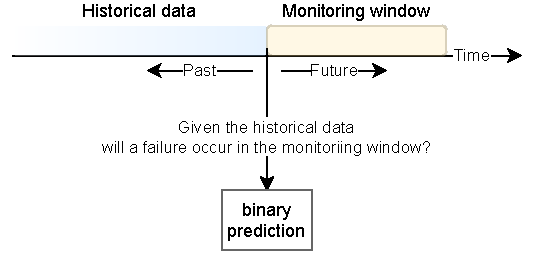
\includegraphics{approaches_failure_prediction_concept.pdf}
\caption{}
\end{subfigure}\\[1ex]
\begin{subfigure}{.5\linewidth}
\centering
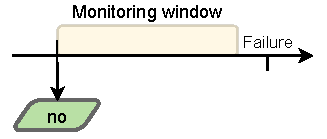
\includegraphics{approaches_failure_prediction_example_neg.pdf}
\caption{}
\end{subfigure}
\begin{subfigure}{.5\linewidth}
\centering
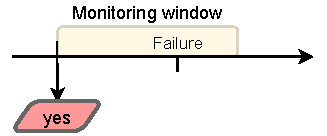
\includegraphics{approaches_failure_prediction_example_pos.pdf}
\caption{}
\end{subfigure}
\caption{Illustration of failure prediction:
        (a) general concept;
        (b) example of negative prediction, i.e. failure won't occur;
        (c) example of positive prediction, i.e. failure will occur.}
\label{fig:approaches_failure_prediction_illustration}
\end{figure}

Failure prediction is an approach where the goal is to make a binary prediction whether a failure will happen in near future --- in a monitoring window.
The concept of failure prediction is illustrated in the Figure 
\ref{fig:approaches_failure_prediction_illustration}.
Failure prediction approach is suitable in cases when there are available data about failures and when there are some patterns that precede the failure --- e.g. when an air compressor raises low pressure alarms before it fails.

\begin{figure}
    \includegraphics[width=.8\textwidth, keepaspectratio]{%
        approaches_failure_prediction_example_windows.pdf}
    \centering
    \caption{Illustration of monitoring, prediction and warning windows.}
    \label{fig:approaches_failure_prediction_example_windows}
\end{figure}

When predicting a failure, the domain problem might require the predictions to be made at least some time prior to the failure, e.g. the technicians have to be informed at least two days ahead in order to be able to schedule and perform the maintenance.
Therefore, a warning window might be specified which marks the minimal time prior to the failure in order for the prediction to be considered useful.
The time period of useful predictions is then called a prediction window and is defined as the time period between $t_F - M$ and $t_F - W$, where $t_F$ is a time stamp of the failure, $M$ is the size of the monitoring window and $W$ is the size of the warning window.
Figure \ref{fig:approaches_failure_prediction_example_windows} illustrates prediction and warning windows.

Failure prediction can be seen as a special case of fault detection where the prediction window are range-based faults.
However, failure prediction has some specifications in modeling and evaluation that differ from the range-based faults detection and thus we describe it as a special approach.

The concept of failure prediction is also used in many other domains such as healthcare, where heart failures are predicted, and it can also be found under name of early fault detection, early prediction of rare event, rare events prediction or rare events classification
\cite{ng2016early,weiss1998learning,ranjan2018dataset,choi2017using}.
In this thesis we will stick to the name failure prediction.

% TODO: add more literature that uses failure prediction and mention what other names they use for warning window etc.

\subsection{Data Specifications}

\begin{table}
	\centering
	\begin{tabular}{|c|c|cccc|c|}
    \hline
    subject id
    & time
    & \multicolumn{4}{|p{4cm}|}{\centering features}
    & failure event\\
    \hline
    subject 1 & 2020-01-01 &          0.1 &         0.05 & $\cdots$ &  34.1 & none \\
	subject 1 & 2020-01-02 &          0.3 &         0.12 & $\cdots$ &  34.2 & none \\
    $\vdots$ & $\vdots$ & $\vdots$ & $\vdots$ & $\ddots$ & $\vdots$ & $\vdots$ \\
    subject 1 & 2020-05-06 &          1.1 &         3.2 & $\cdots$ &  37.5 & none \\
    subject 1 & 2020-05-07 &          1.2 &         3.1 & $\cdots$ &  37.9 & failure A \\
    subject 1 & 2020-05-08 &          0.2 &         0.02 & $\cdots$ &  33.1 & none \\
    subject 1 & 2020-05-09 &          0.3 &         0.05 & $\cdots$ &  33.5 & none \\
    $\vdots$ & $\vdots$ & $\vdots$ & $\vdots$ & $\ddots$ & $\vdots$ & $\vdots$ \\
    subject 1 & 2020-07-29 &          2.5 &         0.21  & $\cdots$ &  35.9 & none \\
    subject 1 & 2020-07-30 &          2.2 &         0.2  & $\cdots$ &  36.1 & failure B \\
    $\vdots$ & $\vdots$ & $\vdots$ & $\vdots$ & $\ddots$ & $\vdots$ & $\vdots$ \\
	\end{tabular}
    \caption{A example of run-to-failure data set for failure prediction.}
    \label{tab:pdm_data_run_to_failure}
\end{table}

Data for training a failure prediction model must contain information about failures.
The data typically consist a condition monitoring data that are continuously collected during time and a failure log --- information when failures happened.
Such data are often called run-to-failure.
An example of run-to-failure data is illustrated in Table \ref{tab:pdm_data_run_to_failure}.
Moreover, it is necessary to have monitoring and warning windows.
However, it is good to note that the monitoring time does not have to be fixed.
Multiple models with different monitoring windows can be built and the choice of the final monitoring window can be made based on how the individual models perform.

\begin{figure}[H]
    \includegraphics[width=\textwidth, keepaspectratio]{%
        approaches_failure_prediction_modeling.pdf}
    \centering
    \caption{Diagram of modeling failure detection as time series
             point-based classification.}
    \label{fig:approaches_failure_prediction_modeling}
\end{figure}

\subsection{Modeling}

% \begin{figure}
%     \includegraphics[width=\textwidth, keepaspectratio]{%
%         approaches_failure_prediction_regression.png}
%     \centering
%     \caption{TODO}
%     \label{fig:approaches_failure_prediction_regression}
% \end{figure}

A failure prediction model can be built using a supervised classification algorithm where the samples in the training data are artificially labelled prior to the failure as positive.
Moreover, the predictions can be smoothed.
The whole modeling process is visualized in Figure
\ref{fig:approaches_failure_prediction_modeling} and described below.

\subsubsection{Artificial Labeling}

The classifier should learn to predict positive samples prior to failures.
Therefore, samples up to $M$ time steps prior to a failure are labeled as positive.
An example of artificial labeling with monitoring window of size 6 is illustrated in the upper part of Figure \ref{fig:approaches_failure_prediction_modeling}.

\subsubsection{Prediction}

The predictions are made point-wise by the trained classifier.
However, it might happen that there occur a single positive prediction among negative predictions due to a noise.
Therefore, the predictions can be smoothed using a rolling window and a positive prediction is assigned at time point $t$ when the ratio of positive predictions in the last $n$ predictions is higher  or equal than a given threshold.
We call the two parameters mentioned above a smoothing window and a smoothing threshold.
In case the classifier is capable of predicting probabilities of classes, the smoothing can be performed on the probabilities before the decision threshold is applied to avoid having two thresholds.

\subsection{Evaluation}
\label{sec:approaches_failure_prediction_evaluation}

In this section we describe how to evaluate the performance of a failure prediction model.
During evaluation we will aim to answer following questions:
\begin{itemize}
    \item What is the probability that the model will detect a failure?
    \item What is the probability that the model will make a false alarm? I.e. makes positive prediction but the failure won't occur in the monitoring window.
\end{itemize}
These questions are in \acrshort{ml} commonly answered by precision and recall metrics.
However, since we have more positive labels than failures due to artificial labeling, it is not straightforward how to use these metrics.
Below, we describe how to use classical precision and recall (described in Section \ref{sec:ml_evaluation}) and range-based precision and recall (described in Section \ref{sec:approaches_fault_detection_evaluation}) to evaluate a failure prediction model.
Next, we describe a modification of precision and recall, reduced precision and recall, introduced by Weiss et al. \cite{weiss1998learning}.
Finally, we propose new precision and recall metrics, a combination of the range-based metrics and the reduced metrics, that we call event-based precision and recall.

\subsubsection{Classical Precision and Recall}
\label{sec:approaches_failure_prediction_evaluation_classical_metrics}

This section describes how to use precision and recall using their standard definition (Section \ref{sec:ml_evaluation}) for failure prediction.

\begin{figure}
    \includegraphics[width=\textwidth, keepaspectratio]{%
        approaches_failure_prediction_evaluation.pdf}
    \centering
    \caption{Illustration of true labels and predictions in failure prediction.}
    \label{fig:approaches_failure_prediction_evaluation}
\end{figure}

As we use artificially created positive labels, we define following: 
\begin{enumerate}
    \item Actual positive samples are samples in the prediction windows, i.e. between $t_F - M$ and $t_F - W$.
    \item Actual negative samples are samples before $t_F - M$.
    \item Samples in the warning window, i.e. between $t_F - W$ and $t_F$, are not omitted from evaluation as they do not represent useful predictions.
\end{enumerate}

Figure \ref{fig:approaches_failure_prediction_evaluation} illustrates what time points are considered as positive and negative and which predictions are considered as \acrshort{tp}, \acrshort{tn}, \acrshort{fp} and \acrshort{fn}.
Recall and precision metrics are then used by their standard definition as:
\begin{align*}
    \text{recall} &= \frac{\text{TP}}{\text{P}},\\
    \text{precision} &= \frac{\text{TP}}{\text{TP} + \text{FP}}.
\end{align*}

\begin{figure}[hbt!]
    \includegraphics[width=.9\textwidth, keepaspectratio]{%
        approaches_failure_prediction_evaluation_recall_con.pdf}
    \centering
    \caption{Different predictions for the same data having the same recall score:
             (\textbf{left}) all of the three failures predicted
             (\textbf{right}) only one failure predicted.}
    \label{fig:approaches_failure_prediction_evaluation_recall_con}
\end{figure}

\begin{figure}[hbt!]
    \includegraphics[width=.75\textwidth, keepaspectratio]{%
        approaches_failure_prediction_evaluation_precision_con.pdf}
    \centering
    \caption{Different positions of two FPs having different severity:
             (\textbf{top}) far from each other
             --- such FPs can be considered as independent;
             (\textbf{middle}) close to each other
             --- the second FP is less serious and the two FPs can be almost
             considered as one;
             (\textbf{bottom}) close to each other and close to the monitoring period
             --- probably not so serious FPs as it might happen that the failure
             was predicted a bit sooner than at $t_F - M$.}
    \label{fig:approaches_failure_prediction_evaluation_precision_con}
\end{figure}

The classical metrics have two major issues:
\begin{itemize}
    \item Recall doesn't reflect how many failures were predicted.
    Figure \ref{fig:approaches_failure_prediction_evaluation_recall_con} shows examples of two models whose predictions have same recall score but they successfully predicted different number of failures.
    \item Precision doesn't reflect how close FPs are to each other.
    Figure \ref{fig:approaches_failure_prediction_evaluation_precision_con} shows examples of three series all having two \acrshort{fp}s but possibly having different importance in practice, e.g. two consecutive FPs may be treated as one FP whereas two FPs far from each other should count as two FPs.
\end{itemize}
Below, we describe three other types of precision and recall metrics that might mitigate these issues.

\subsubsection{Range-based Precision and Recall}

Failure prediction can be evaluated using range-based precision and recall as described in Section \ref{sec:approaches_fault_detection_evaluation} by taking the prediction windows as real fault (anomaly) ranges and consecutive positive predictions as predicted ranges.
Setting a non-zero existence weight $\alpha$ to the detection score of the range-based metrics solves the first issue mentioned above --- recall not reflecting how many failures were predicted.

\subsubsection{Reduced Precision and Recall}

Weiss et al. introduced in 1998 evaluation metrics called reduced precision and recall for prediction of rare events in time series \cite{weiss1998learning} which is a problem identical to failure prediction.
The main idea of the reduced metrics is to use the number of events (failures) instead of positive samples, use the number of predicted events instead of TP and use discounted FP instead of FP.

\paragraph{P $\rightarrow$ TotalEvents}
The total number of events (failures) is used instead of positive samples.
This means that for every prediction window consisting of $M - W$ samples there is one even, i.e. total number of events is equal to dividing the number of positives by the size of a prediction window.

\begin{figure}
    \centering
    \begin{subfigure}{.45\textwidth}
        \centering
        \includegraphics[width=.7\linewidth]{%
            approaches_failure_prediction_evaluation_failure_predicted.pdf}
        \caption{Failures predicted}
      \label{fig:approaches_failure_prediction_evaluation_failure_predicted}
    \end{subfigure}%
    \begin{subfigure}{.45\textwidth}
        \centering
        \includegraphics[width=.7\linewidth]{%
            approaches_failure_prediction_evaluation_failure_not_predicted.pdf}
        \caption{Failures not predicted}
        \label{fig:approaches_failure_prediction_evaluation_failure_not_predicted}
    \end{subfigure}
    \caption{Illustrations of events (failures) being and not being predicted}
\end{figure}

\paragraph{TP $\rightarrow$ EventsPredicted}
The true positives are replaced by the number of predicted events.
The event is considered as predicted when there is at least one positive prediction in its prediction window, i.e. at least $W$ and at most $M$ time steps prior to the event.
Figures \ref{fig:approaches_failure_prediction_evaluation_failure_predicted} and \ref{fig:approaches_failure_prediction_evaluation_failure_not_predicted} illustrate examples of events being predicted and not being predicted, respectively.

\begin{figure}
    \includegraphics[width=.75\textwidth, keepaspectratio]{%
        approaches_failure_prediction_evaluation_discounted_fp.pdf}
    \centering
    \caption{Illustration of calculating DiscountedFP.}
    \label{fig:approaches_failure_prediction_evaluation_discounted_fp}
\end{figure}

\paragraph{FP $\rightarrow$ DiscountedFP}
Every positive prediction has a meaning that an event (failure) will happen in the monitoring window.
If there are two consecutive positive predictions, the latter prediction can be considered as having lesser severity as the two consecutive predictions can be regarded as one false alarm.
Therefore, Weiss et al. define calculate as the number of complete, non-overlapping, monitoring windows associated with a false positive \cite{weiss1998learning}.
For example when having monitoring window of size 10, two consecutive false positives will produce a discounted FP of 1.1, i.e. 1 for the first prediction plus 0.1 for the second.
If the there is a false positive at time point $t$ and a false positive at time point $t + 5$, then the discounted FP for these two false positives will be equal 1.5.
Figure \ref{fig:approaches_failure_prediction_evaluation_discounted_fp} illustrates how discounted FP is calculated in three different scenarios.

The reduced precision and recall metrics are then defined as:
\begin{align*}
    \text{reduced recall} &= \frac{\text{EventsPredicted}}{\text{TotalEvents}},\\
    \text{reduced precision} &=
    \frac{\text{EventsPredicted}}
    {\text{EventsPredicted} + \text{DiscountedFP}}.
\end{align*}

Reduced recall is then identical to range-based precision when setting $\alpha = 1$, i.e. taking into account only the existence of a positive prediction in the prediction window.

\subsubsection{Event-based Precision and Recall}

Above, we described how range-based and reduced metrics can be used for failure prediction.
In this section, we propose a combination of the range-based and the reduced metrics.
The combination consists in taking the reduced metrics replacing the number of events predicted by a sum of detection scores from the range-based metrics.
We call such metrics event-based precision and recall and define it as follows:
\begin{align*}
    \text{event-based recall} &= \frac{\sum\text{DetectionScore}}{\text{Events}},\\
    \text{event-based precision} &=
    \frac{\sum\text{DetectionScore}}
    {\sum\text{DetectionScore} + \text{DiscountedFP}}.
\end{align*}
where $\sum\text{DetectionScore}$ is a sum of detection scores for all the prediction windows.
\section{Remaining Useful Life Prediction}
\label{sec:approaches_prognostics}

\Acrfull{rul} prediction is a \gls{pdm} approach where the goal is to predict the time left until the subject is still able to perform its intended function, i.e. until a failure occurs.
This section is structured as follows.
In Section \ref{sec:approaches_rul_motivation} we give a motivation why and when to predict \acrshort{rul} instead of using fault detection or failure prediction approaches.
In Section \ref{sec:approaches_rul_approaches} we describe and compare two different modeling approaches to \acrshort{rul} prediction --- \acrshort{hi}-based \acrshort{rul} prediction and direct \acrshort{rul} prediction.
The two approaches fundamentally differ in how \acrshort{rul} is predicted.
However, they still provide the same output --- the \acrshort{rul} of the subject --- and thus can be evaluated the same way.
Therefore, in the Section \ref{sec:approaches_rul_evaluation} we describe how to evaluate the \acrshort{rul} prediction independently on the chosen modeling approach.

\subsection{Motivation}
\label{sec:approaches_rul_motivation}

An accurate long term \acrshort{rul} prediction can significantly help in scheduling the maintenance actions in comparison with fault detection or failure prediction approaches.
Imagine a situation of having a large amount of subjects which started operating at the same time --- for example a fleet of one hundred wind turbines.
If the turbines were operating under similar conditions it might happen that they will all tend to fail after similar amount of time of operation --- e.g. after two years.
Both fault detection and failure prediction approaches would then notify that all the wind turbines are faulty (or are going to fail soon) at a similar time shortly before the failures, let's say one week ahead.
However it might be impossible to schedule maintenance actions for all the wind turbines at that time point because only two wind turbines can be maintained per day and there is one hundred of wind turbines about to fail in one week.
With an accurate \acrshort{rul} prediction, on the other hand, one can continuously have information about when each individual subject is going to fail.
If the \acrshort{rul} is then similar for many subjects the maintenance actions can be scheduled more in advance so that all the subjects are maintained in advance.
However, an accurate \acrshort{rul} prediction is typically possible only in certain domains and only when having the right type of data.

\Acrshort{rul} prediction is typically done on subjects which have an ongoing continuous degradation that can be well quantified --- for example a turbine bearing deterioration.
The failure then can be either a complete inability of the subject to operate (e.g. the wind turbine shuts down) or it can be a state when the subject is no longer capable of safe operation or of operation at enough quality --- e.g. a maximum capacity of a battery reaches 40 \% of the designed capacity\footnote{In such cases the failure is often rather called an end of life (EoL). However, as it principally represents the same thing we will stick to the naming convention of failure.}.
In such cases it is common to predict \acrshort{rul} during the whole lifetime of the subject (e.g. every day or week) \cite{miao2013remaining}.
In other cases, however, the subject might operate under stable, healthy, conditions without any sings of wear until a fault occurs which triggers the degradation process --- the fault grows in severity (as illustrated in the beginning of this chapter in Figure \ref{fig:approaches_intro_health_stages}).
In such cases the \acrshort{rul} can be predicted over the whole lifetime as well but it might happen that the prediction would be highly inaccurate until the fault occurs.
Therefore, the \acrshort{rul} prediction can 
start after the fault (or anomaly) is detected\footnote{assuming the fault is detected early enough so that the \acrshort{rul} prediction is useful} \cite{lei2018machinery} and thus providing an estimation of the fault's severity.

\subsection{Approaches}
\label{sec:approaches_rul_approaches}

We identified two different modeling approaches to \acrshort{rul} prediction --- direct RUL prediction and HI-based RUL prediction\footnote{HI --- health indicator}.
In this section we describe and compare the two approaches.

% Before we proceed to their description, however, we want to shortly comment on the naming of the approaches.
% There is very few literature that mentions the existence of the both approaches.
% Typically only one of the approaches is used (or described) and it is simply referred to both of them as \acrshort{rul} prediction \cite{miao2013remaining, hu2012ensemble, klausen2018novel,  yang2016health}.
% The first approach, the \acrshort{hi}-based \acrshort{rul} prediction, can be considered as a classical approach to \acrshort{rul} prediction as there is much more literature using this approach and 

% The first approach consists in construction of a \acrfull{hi} from the condition monitoring data, forecasting its future values and predicting when the \acrshort{hi} crosses a predefined failure threshold.
% In this approach it is common that a separate model is build for every subject and the model is updated with each new health indicator value \cite{lei2018machinery}.
% The second approach consists in direct prediction of the \acrshort{rul} from the condition monitoring data using a regression model.
% The regression model is trained on historical run-to-failure data of subjects from which their \acrshort{rul} is calculated.
% Unfortunately, 
% % The first approach, utilizing the \acrshort{hi}, is sometimes referred to as prognostics  \cite{lei2018machinery, lee2014prognostics} but the definition of prognostics is that it is a \acrshort{rul} prediction \cite{lei2018machinery}.
% % The second approach is sometimes referred to as regression approach to \acrshort{rul} prediction \cite{babu2016deep} but as will be described later in this section even the first approach can utilize regression models.
% The only work we found that tries to distinguish between the approaches \cite{jia2018review} calls them "Unsupervised Prognosis" and "Supervised RUL Prediction".
% However, that is highly ambiguous naming as first approach can utilize supervised learning algorithms as well and as the prognosis and \acrshort{rul} prediction are equivalent.
% Therefore, we decide to call the two approaches an \acrshort{hi}-based \acrshort{rul} prediction and a direct \acrshort{rul} prediction.
% We describe and compare both of the approaches in more detail in Section  \ref{sec:approaches_rul_approaches}.

\subsubsection{Direct \acrshort{rul} Prediction}
\label{sec:approaches_rul_direct}

\begin{table}
	\centering
	\begin{tabular}{|c|c|ccc|c|c|c|}
    \hline
    subject id
    & time
    & \multicolumn{3}{|p{3cm}|}{\centering features}
    & failure
    & \textbf{RUL}\\
    \hline
    subject A & 2020-01-01 &          0.1 & $\cdots$ &  34.1 & 0 & 127\\
	subject A & 2020-01-02 &          0.3 & $\cdots$ &  34.2 & 0 & 126\\
    $\vdots$ & $\vdots$ & $\vdots$ & $\ddots$ & $\vdots$ & $\vdots$ & $\vdots$\\
    subject A & 2020-05-05 &          1.1 & $\cdots$ &  37.5 & 0 & 2\\
    subject A & 2020-05-06 &          1.1 & $\cdots$ &  37.5 & 0 & 1\\
    subject A & 2020-05-07 &          1.2 & $\cdots$ &  37.9 & 1 & 0\\
    \hdashline
    subject B & 2020-01-01 &          0.2 & $\cdots$ &  33.1 & 0 & 89\\
    subject B & 2020-01-02 &          0.3 & $\cdots$ &  33.5 & 0 & 88\\
    $\vdots$ & $\vdots$ & $\vdots$ & $\ddots$ & $\vdots$ & $\vdots$ & $\vdots$\\
    subject B & 2020-03-29 &          2.5 & $\cdots$ &  35.9 & 0 & 1\\
    subject B & 2020-03-30 &          2.2 & $\cdots$ &  36.1 & 1 & 0\\
    \hline
	\end{tabular}
    \caption{Example of calculating the \acrshort{rul} values from the run-to-failure data.}
    \label{tab:pdm_data_run_to_failure}
\end{table}

Direct \acrshort{rul} prediction is suitable when there are available run-to-failure data for at least several subjects.
The approach consists in training a regression model on the run-to-failure data where the regressands (features) can be any known data about the subject at the time of the prediction and the regressor (the predicted value) is the \acrshort{rul} retrospectively calculated from the run-to-failure data.
The calculation of the RUL is typically done as follows --- at the time of the failure, $T$, the RUL is equal to 0, at time $T-1$ the RUL is equal to 1, at $T-2$ the RUL is equal to 2 and so on.
Table \ref{tab:pdm_data_run_to_failure} shows an example of run-to-failure data set and calculating of the RUL.

As described in the previous section, the subjects might operate under stable and healthy conditions until a fault occurs which triggers the degradation process.
In that case the RUL prediction might be very inaccurate at the early stage of the subject's operation where it might be hard to distinguish between e.g. RUL of 200 days and 170 days.
Therefore in some works limiting of the \acrshort{rul} values with an upper bound is suggested \cite{jayasinghe2018temporal} --- e.g. all the RUL values above 130 are set to 130  see Figure \ref{fig:approaches_rul_clipping} for illustration).
The authors in \cite{jayasinghe2018temporal} conclude that such clipping might result in better performance in terms of root mean squared error metric.
However, as will be discussed in Section \ref{sec:approaches_rul_evaluation} the RMSE metric might be unsuitable for evaluation of RUL prediction performance and thus it is questionable whether this RUL clipping helps the overall performance of the model.

\begin{figure}
    \centering
    \includegraphics[width=.6\textwidth, keepaspectratio]{%
        approaches_rul_clipping.png}
    \caption{Illustration of limiting RUL with an upper bound \cite{jayasinghe2018temporal}.}
    \label{fig:approaches_rul_clipping}
\end{figure}

\begin{figure}
    \centering
    \includegraphics[width=.6\textwidth, keepaspectratio]{%
        approaches_rul_bayesian.png}
    \caption{Illustration of RUL prediction with a Bayesian LSTM neural network  \cite{louw2018remaining}.}
    \label{fig:approaches_rul_bayesian}
\end{figure}

Promising results of direct RUL prediction have been achieved with recurrent and convolutional neural networks in various domains such as wind turbines or bearings \cite{mahamad2010predicting, babu2016deep}.
In recent years, Bayesian neural networks are gaining on interest in direct RUL prediction as they can predict a \gls{pdf} instead of single value predictions \cite{peng2019bayesian, louw2018remaining}.
The mean of the \gls{pdf} can then be used as the predicted RUL and a confidence interval can be calculated and used as a form of uncertainty --- which might be very valuable for the end users as a supportive information about the prediction.
Figure \ref{fig:approaches_rul_bayesian} illustrates prediction of \gls{rul} with a Bayesian LSTM neural network.

In some literature, the direct \acrshort{rul} prediction approach is considered as having relatively low capability of predicting the \acrshort{rul} since a linear relationship between the \acrshort{rul} and the condition monitoring data is established \cite{jia2018review}.
% However, we must emphasize that the linear relationship holds only when using raw data and a linear model.
% When a more complex model such as SVM with higher degree polynomial kernel or an artificial neural network is used or when some feature engineering is performed (e.g. squared age of the subject is used as a feature), the mentioned linear relationship no longer holds.

\subsubsection{\acrshort{hi}-based \acrshort{rul} Prediction}
\label{sec:approaches_rul_hi_based}

The \acrshort{hi}-based \acrshort{rul} prediction approach is suitable in cases when there is available a \acrfull{hi} that directly represents the subject's health state and a predefined failure threshold.
The failure of the subject is then considered as the time point when the \acrshort{hi} crosses the failure threshold.
A typical example of such case are batteries where the health indicator can be their current maximal capacity and the failure threshold can be a ratio of the designed maximal capacity (e.g. 30 \%).
% Another example are bearings where the health indicator can be root mean square of vibration data and the failure threshold can be some maximal permissible vibration level --- e.g. ISO norm \cite{iso_mechanical} even defines permissible thresholds for some bearings.
The \acrshort{rul} prediction then consists in building a model that forecasts future values of the \acrshort{hi} and in identifying the time point when the HI crosses the failure threshold.
The RUL is then calculated as the time difference between the identified time point of the crossing and the current time point.

\begin{figure}
    \centering
    \includegraphics[width=\textwidth, keepaspectratio]{%
        approaches_rul_prognostics_example.png}
    \caption{Illustration of \acrshort{hi}-based \acrshort{rul} prediction.
             The red dashed line represents a failure threshold (FT), the blue line
             represents a health indicator up to a current time point (green dot), the green
             line shows a prediction of the health indicator in the future and
             the red line represents the actual future values of the health indicator.
             \cite{lei2018machinery}.}
    \label{fig:approaches_rul_prognostics_example}
\end{figure}

The forecasted \acrshort{hi} is commonly in a form of a \acrfull{pdf} which tends to have higher variance the farther to the future the \acrshort{hi} is predicted \cite{saxena2010metrics}.
In case of predicting the \gls{pdf} of the HI the failure can be defined as the time point when the mean of the \acrshort{pdf} crosses the failure threshold.
Figure \ref{fig:approaches_rul_prognostics_example} illustrates the forecasting of the \acrshort{hi} with a \acrshort{pdf}.

The HI forecasting techniques can be divided into two categories:
\begin{itemize}
    \item model-based techniques;
    \item machine learning techniques;
\end{itemize}

\begin{figure}
    \centering
    \includegraphics[width=.7\textwidth, keepaspectratio]{%
        intro_pdm_battery_degradation.jpg}
    \caption{Finding an empirical model for degradation of battery capacity 
             \cite{miao2013remaining}.}
    \label{fig:approaches_rul_battery}
\end{figure}

\paragraph{Model-based Techniques}
The model-based techniques are based on the existence of an underlying physical or statistical model that describes the degradation process of the subject.
Such physical or statistical models can be either apriori known or empirically observed from the available data.
For example the capacity of the batteries can be commonly fitted by an exponential model \cite{he2011prognostics} --- see Figure \ref{fig:approaches_rul_battery} for illustration.
The physical and statistical models have typically parameters which are estimated from the currently available HI data of the subject (the parameters are estimated for each subject separately).
In other words the forecasting at time point $t$ is done by a model with parameters estimated based on the HI data up to time point $t$.

\paragraph{ML Techniques}
The AI techniques, on the other hand, do not require any domain knowledge about the degradation process but rather build a model that learns the degradation patterns from the previous HI data points by itself.
A simple technique can be using a regression model that takes time as the regressand and the HI as the regressor \cite{yoo2018novel}.
More advanced techniques include for example a recurrent neural networks which can be trained to time series prediction, i.e. output future values of the HI based on previous values \cite{zhang2018long}.

% TODO: Uber extreme forecasting

A big benefit of HI-based RUL prediction over the direct RUL prediction is that there is no need for run-to-failure data.
The unavailability of run-to-failure data is common in many domains such as aviation where the subjects simply cannot operate until a failure mostly from safety reasons \cite{saxena2010metrics}.
On the other hand, the downside of the HI-based RUL prediction is that there has to be a well defined health indicator and failure threshold.

\subsection{Evaluation}
\label{sec:approaches_rul_evaluation}

In this section, we describe how to evaluate the performance of a RUL prediction model.
We will use the following notation:
\begin{itemize}
    \item $N$ --- number of subjects;
    \item $n \in [1, N]$ --- index of a n-th subject;
    \item $t \in [1, T_n]$ --- time index of n-th subject's observations, where $t=1$ is the first observation and $t=T_n$ is the time stamp of the failure;
    \item $\text{RUL}_n(t)$ --- actual \gls{rul} of n-th subject at time $t$;
    \item $\widehat{\text{RUL}}_n(t)$ --- predicted \gls{rul} of n-th subject at time $t$;
    \item $W$ --- warning time;
    \item $\text{EoUP}_n = T_n-W$ --- \acrfull{eoup}, the last time stamp of useful predictions, i.e. not yet in the warning window.
\end{itemize}
The warning time has the same meaning as in failure prediction --- some lead time before the failure of the subject might be necessary so that the maintenance action can be scheduled and performed.
Therefore, we will exclude the time points between $T-W$ and $T$ from the evaluation.

% The performance of \acrshort{rul} prediction can be evaluated on four levels:
% \begin{enumerate}
    
%     \item single prediction level --- what is the error of the prediction from the actual RUL?
    
%     \item \acrshort{rul} level --- what is a typical error of predicting a specific actual \acrshort{rul} value? (e.g. how accurate are the predictions when actual RUL value is 100 days vs 10 days);
%     % \item relative \acrshort{rul} level --- what is a typical error of the model when
%     %       predicting a specific actual \acrshort{rul} value (e.g. a mean error
%     %       of predictions for the actual \acrshort{rul} of 100 days is 10 days);
    
%     \item subject level --- how accurate is the model in predicting \acrshort{rul} of a specific subject?;
    
%     \item data set level --- what is the overall performance of the predictions on the whole data set, e.g. on a fleet of subjects?;

% \end{enumerate}
% Below we will describe various evaluation metrics and techniques and we will describe how they can be used for evaluation at the different levels mentioned above.

% The \acrshort{rul} predictions are made for every subject while the predicted values 
% Each prediction is made for a specific time stamp of a specific subject.

\subsubsection{Classical Metrics}

\Acrshort{rul} prediction is in context of \acrshort{ml} a regression task --- the goal is to predict a continuous variable.
Thus, classical regression metrics such as MAE, RMSE or MAPE can be used.
However, it is not straightforward how to use them from two reasons.
First, we should omit the predictions made in the warning window, the predictions after \acrshort{eoup}.
Second, we can calculate the mean error either over subjects or over individual samples.

An absolute error, squared error and absolute percentage error for n-th subject can be calculated as:
\begin{align*}
    \text{AbsoluteError}_n &= \sum_{t=1}^{\text{EoUP}_n}\left|\text{RUL}_n(t) - \widehat{\text{RUL}}_n(t)\right|,\\
    \text{SquaredError}_n &= \sum_{t=1}^{\text{EoUP}_n}{(\text{RUL}_n(t) - \widehat{\text{RUL}}_n(t))^2},\\
    \text{AbsolutePercentageError}_n &= \sum_{t=1}^{\text{EoUP}_n}\left|\frac{\text{RUL}_n(t) - \widehat{\text{RUL}}_n(t)}{\text{RUL}_n(t)}\right|.\\
\end{align*}
In general, we will denote the error of the n-th subject as Error$_n$.
The mean of the errors can be then calculated either over subjects or over samples:
\begin{align*}
    \text{mean error over subjects} &= \frac{1}{N}\sum_{n=1}^{N}\frac{\text{Error}_n}{\text{EoUP}_n},\\
    \text{mean error over samples} &= \frac{1}{\sum_{n=1}^N{{\text{EoUP}_n}}}\sum_{n=1}^{N}{\text{Error}_n}.\\
\end{align*}

Mean absolute percentage error (MAPE) over samples can be then calculated as:
\begin{align*}
    \text{MAPE} = \frac{1}{\sum_{n=1}^N{{\text{EoUP}_n}}}\sum_{n=1}^{N}{\sum_{t=1}^{\text{EoUP}_n}\left|\frac{\text{RUL}_n(t) - \widehat{\text{RUL}}_n(t)}{\text{RUL}_n(t)}\right|}
\end{align*}
The metrics such as MAE and RMSE are then calculated analogically.

% Typically, the lower the actual \acrshort{rul} is the more accurate the predictions should be --- e.g. it is much less severe error if the actual \acrshort{rul} is 200 days and the prediction is 220 days in comparison with an actual \acrshort{rul} being 5 days and the prediction being 25 days.
% This exactly reflects MAPE metric which scales the errors accordingly to the actual predicted value.

\subsubsection{Prognostic Horizon}

\begin{figure}
    \centering
    \includegraphics[width=\textwidth, keepaspectratio]{%
        approaches_rul_evaluation_prognostic_horizon.pdf}
    \caption{Illustration of prognostic horizon.}
    \label{fig:approaches_rul_evaluation_prognostic_horizon}
\end{figure}

Prognostic horizon is an evaluation metric specifically tailored for \acrshort{rul} prediction proposed by Saxena et al. \cite{saxena2010metrics}.
It aims to answer the following question: What time ahead of the failure are the predictions within a prespecified bound around the actual \acrshort{rul} for one specific subject?
The prognostic horizon is defined as the time difference between the time of failure ($T_n$) and the first time index from which all the future predictions are within the boundaries specified by parameter $\alpha$.
For the n-th subject the prognostic horizon (PH) with parameter $\alpha$ is defined as:
\begin{align*}
    \text{PH}_{\alpha, n} &= T - \min\left\{i|
        \forall t, t \geq i : \widehat{\text{RUL}}_n(t) \in [\text{RUL}_n(t) - \alpha, \text{RUL}_n(t) + \alpha]
  \right\}.
\end{align*}
Figure \ref{fig:approaches_rul_evaluation_prognostic_horizon} illustrates the calculation of prognostic horizon on predictions for one subject.

For evaluation of multiple subjects, \acrfull{mph}$_\alpha$ can be used as:
\begin{align*}
    \text{MPH}_\alpha = \frac{1}{N}\sum_{n}{\text{PH}_{\alpha, n}}
\end{align*}

\subsubsection{Metrics Relative to RUL}

% All the above mentioned metrics produce a single score.
% Therefore, when we obtain e.g. a score RMSE equal to 20, we do not know whether there were high errors at the beginning a

It might happen that the RUL prediction model has relatively high errors at high RUL values compared to the errors at low RUL values.
Therefore, we can calculate the errors only for RUL values lower than a certain fixed value, for example calculate MAPE only for RUL values lesser than 40.
We define a mean absolute percentage error up to RUL values equal to $k$ (MAPE@k) as:
\begin{align*}
    \text{MAPE@k} = \frac{1}{\sum_{n=1}^N{{\left(\text{EoUP}_n - k - 1 \right)}}}\sum_{n=1}^{N}{\sum_{t=k}^{\text{EoUP}_n}\left|\frac{\text{RUL}_n(t) - \widehat{\text{RUL}}_n(t)}{\text{RUL}_n(t)}\right|}
\end{align*}
Metrics such as MAE@k, RMSE@k can be then defined analogically.

In RUL prediction, we might be interested in how the model performs at relatively to the actual RUL values, i.e. we might want to obtain one score for every actual RUL value.
Therefore, instead of calculating a mean score over all the samples, we can calculate a mean score over all subjects at a various RUL values.
MAPE at different RUL values is defined as follows:
\begin{align*}
    \text{MAPE(RUL)} = \sum_n \frac{\text{RUL} - \widehat{\text{RUL}}_n(T_n - \text{RUL})}{\text{RUL}}.
\end{align*}
The metrics MAE, RMSE and others can be then defined analogically.

% TODO
% TODO

% Saxena et al. proposed a metric called relative accuracy \cite{saxena2010metrics} which measures the accuracy of the \acrshort{rul} prediction at a relative \acrshort{rul} value:
% \begin{align*}
%     \text{RelativeAccuracy}_\lambda = 1 - \frac{|y_{\lambda T} - \hat{y}_t|}{y_t}
% \end{align*}
% where $t_\lambda = \lambda T, \lambda \in [0, 1]$

% \begin{figure}
%     \centering
%     \includegraphics[width=\textwidth, keepaspectratio]{%
%         approaches_prognostics_relative_accuracy.pdf}
%     \caption{Relative accuracy}
%     \label{fig:approaches_prognostics_relative_accuracy}
% \end{figure}


\begin{figure}[H]
    \centering
    \includegraphics[width=\textwidth, keepaspectratio]{%
        approaches_rul_prediction_optimistic.pdf}
    \caption{Illustration of optimistic and pessimistic predictions.}
    \label{fig:approaches_rul_prediction_optimistic}
\end{figure}

\begin{figure}[H]
    \centering
    \includegraphics[width=.8\textwidth, keepaspectratio]{%
        approaches_rul_asymmetric_scoring.png}
    \caption{Asymmetric weighting function for late and early predictions \cite{saxena2008damage}.}
    \label{fig:approaches_rul_asymmetric_scoring}
\end{figure}

\subsubsection{Asymmetric Weighting}

When the prediction is not perfect, i.e. $\text{RUL} \neq \widehat{\text{RUL}}$, it can be either late (optimistic) if $\text{RUL} > \widehat{\text{RUL}}$ or early (pessimistic) if $\text{RUL} < \widehat{\text{RUL}}$.
Figure \ref{fig:approaches_rul_prediction_optimistic} illustrates RUL predictions for one subject and highlights what predictions are late and which are early.
The late predictions might bring a risk that the subject fails before the maintenance is performed.
Therefore, the early predictions are typically better since the subject is in the worst case maintained earlier than it would have to be.

In \cite{nectoux2012pronostia} and \cite{saxena2008damage} the authors suggest using an asymmetric weighting function for weighting the prediction errors.
The main idea is to give higher weight to the late predictions in comparison with the early ones.
The asymmetric weighting function $\varphi$ can be for example defined as
\begin{align*}
    \varphi(d) &= \begin{cases}
            -d &\text{ if } d < 0\\
            2d &\text{ if } d \geq 0
    \end{cases}
\end{align*}
where $d$ is the difference between the predicted RUL and actual RUL, i.e. $d = \widehat{\text{RUL}} - \text{RUL}$.
Figure \ref{fig:approaches_rul_asymmetric_scoring} illustrates the above defined asymmetric weighting function.

The weighting function $\varphi$ can be then used in the classical regression metrics.
We define a mean asymmetrically weighted percentage error (MAWPE) with an asymmetric scoring function $\varphi$ as:
\begin{align*}
    \text{MAWPE}_\varphi &= \frac{1}{\sum_{n=1}^N{{\text{EoUP}_n}}}\sum_{n=1}^{N}{\sum_{t=1}^{\text{EoUP}_n}\left|\varphi\left(\frac{\text{RUL}_n(t) - \widehat{\text{RUL}}_n(t)}{\text{RUL}_n(t)}\right)\right|} \\
\end{align*}
The usage of the asymmetric weighting function in other metrics is then analogical.

The asymmetry can be also applied in prognostic horizon where instead of a single parameter $\alpha$ (defining the width of the bound) two parameters $\alpha^+$ and $\alpha^-$ can be used which define the lower and the upper boundary, respectively.
\input{chapters/approaches/summary}


\chapter{Experiments}
\label{chapter:experiments}

In this chapter we describe experiments conducted on real-world publicly available \gls{pdm} data sets.
There are two main goals of the experiments:
\begin{itemize}
    \item demonstrate the approaches to \gls{pdm} utilizing \gls{ml} techniques;
    \item compare the different evaluation metrics that can be used within each approach.
\end{itemize}
For each of the approaches we conduct one experiment --- totaling in three experiments.

Though there is not enough publicly available data sets to make a robust comparison of the metrics, we can conduct each experiment on one carefully selected data set, suitable for the given approach, and compare the metrics from two aspects:
\begin{itemize}
    \item model selection --- Do evaluation metrics differ in how they rank different models for the task related to the data set?
    \item interpretability and practical value --- How can the evaluation metrics be interpreted by a domain expert? Does the evaluation bring practical value for the task related to the data set? For example do the metrics clearly express what the probability of predicting a failure or detecting a fault is?
\end{itemize}

As the approaches and the evaluation metrics are different, every experiment has slightly different experiment design.
The general design of the experiments can be, however, summarized as follows:
\begin{enumerate}
    \item candidate models selection --- use multiple evaluation metrics to select a set of candidate models from a larger amount of built models, e.g. select best ranked model by every metric, and discuss how the models agree in models' ranking;
    \item candidate models comparison --- compare the candidate models, e.g. using PR analysis, and discuss which model might be the most suitable model for the given task;
    \item performance interpretability --- discuss what will the model's performance in practice be.
\end{enumerate}

This chapter is organized as follows.
In Section \ref{sec:experiments_implementation} we describe implementation of the experiments including chosen technologies and the experiments' reproducibility.
In Sections \ref{sec:experiments_fault_detection}, \ref{sec:experiments_failure_prediction} and \ref{sec:experiments_rul} we describe the three conducted experiments, respectively.
Each experiment consists of sections:
\begin{itemize}
    \item data set description,
    \item task definition,
    \item design of experiment,
    \item results and
    \item discussion.
\end{itemize}

\section{Implementation}
\label{sec:experiments_implementation}

The full implementation of the experiments is available as a GitHub repository\footnote{\url{https://github.com/datamole-ai/predictivemaintenancethesis}}.
In this section, we provide a brief overview about the implementation details.

\subsection{Technologies}

We implemented the experiments as Jupyter notebooks \cite{jupyter} in Python using standard Python libraries for machine learning, scientific computations, and visualizations including Scikit-learn \cite{scikit-learn}, NumPy \cite{numpy}, SciPy \cite{2020SciPy-NMeth}, Matplotlib \cite{matplotlib}, Seaborn \cite{seaborn}, XGBoost \cite{xgboost} and Pandas \cite{pandas}.
For the calculation of range-based precision and recall metrics we used a python implementation the authors of \cite{tatbul2018precision} provide at GitHub \cite{tsmetric}.
Moreover, for the calculation of \acrshort{auprg} we used pyprg package \cite{prg}.

\subsection{Hardware}

We ran the experiments on a computational cluster using 256 GB of RAM and 32 CPU cores of AMD Opteron 6344 CPU units provided by Datamole\footnote{\url{www.datamole.cz}}.

% \subsection{Implementation Details}

% TODO

% Scikit-learn \cite{scikit-learn} is one of the most commonly used Python libraries for machine learning which contains many standard classification and regression algorithms and TODO.
% In \gls{pdm} data sets we often operate with the data for each subject separately, e.g. artificial labeling in failure prediction or calculating e.g. rolling features should be done for each subject separately.
% Therefore, we implement a wrapper class over a scikit-learn's 

% All the evaluation metrics are available as standalone functions compatible with 
% All the experiments are are provided as a GitHub repository (TODO: cite).
% The implementation includes downloading the data from the web,
% preprocessing and data transformation, and all the evaluation metrics described
%  in the previous chapter.
% The experiments thus are reproducible and extensible, and their parts
% are reusable in other works.\markbelow{c}{
%     This section might be extended with the description of the Python library
%     - if it will be part of the Work.
% }

% % Each experiment also contains script for downloading the data 

% The parts of the experiments where algorithms dependent on a random seed (e.g. a random search algorithm for optimizing hyperparameters) use a hardcoded value of the seed.

% The experiments are completely reproducible.

% sklearn model for data in series format
% implementation of various metrics and series_scorer wrapper


\subsection{Reproducibility}

Each experiment is completely reproducible.
We use Poetry package manager \cite{poetry} to ensure that the same versions of Python libraries we used can be installed for reproducing the experiments.
Our GitHub repository thus contains a \texttt{pyproject.toml} and \texttt{poetry.lock} files which can be used to install all the Python packages at the same version we used.
We used a fixed random seed in all parts of code that depend on randomness so that reproducing the experiments always yields the same results.
Reproducing each experiment then consist in running a Jupyter notebook which contain code for downloading the publicly available data set, preprocessing of the data and all the other steps of the experiments such as modeling and visualizing the results.
\section{Experiment --- Fault Detection in Scania Trucks}
\label{sec:experiments_fault_detection}

Fault detection is an approach where the goal is to build a model that detects faulty behaviour, malfunction, of the subject.
It can be modeled as a binary classification or an anomaly detection --- depending on whether health labels are available or not.
It is suitable in cases when there are no or insufficient data about actual failures, i.e. breakdowns, of the subjects.
In this section we describe an experiment where we demonstrate this approach and compare its evaluation metrics on one real-world data set.

The data used for building a fault detection model can contain either point-based or range-based faults, i.e. faults with no temporal location or faults located in time and lasting for a certain period of time (for more details see Section \ref{sec:approaches_fault_detection_data}).
Since detection of range-based faults is partly similar to failure prediction approach, which we demonstrate in the following experiment, we focus in this experiment on fault detection of point-based faults.

For the purpose of our experiment we choose a data set containing point-based faults in air pressurized system of Scania trucks \cite{Dua:2019}.
We choose this data set because its authors clearly define an objective function --- a cost function assigning costs to false alarms and missed faults (FPs and FNs) expressed in the amount of dollars.
The authors then clearly define the task as to build a model that minimize this cost function.
The cost function allows us to demonstrate how decision threshold of the built classifier can be selected in practice.

\subsection{Data Set Description}

The data set we use in this experiment contains condition monitoring data and point-based faults in an air pressure system of heavy Scania trucks \cite{Dua:2019}.
It consists of 76000 records and 171 columns where each row represents one truck with the first column containing a binary health label (positive class represents a fault) and the next 170 columns containing anonymized features.
The provided data are  already split into training and testing set where the training set contains 60000 records and the testing set contains 16000 records.
Both the sets are highly imbalanced --- the ratio of positive classes to the total amount of records is approximately 1.67 \% in the training set and 2.34 \% in the testing set.

\paragraph{Preprocessing}

The data set is provided partially preprocessed in a form of two CSV files, one for training set and one for testing set.
All the features are numerical of which some of them are provided already binned --- i.e. split to a finite number of intervals. 
There are some missing values in multiple feature columns which we impute by a mean of each column in the training data\footnote{Note that it is very important not to impute missing values by a mean values of the whole data set as that would contaminate the data training data with the information from the testing data.}.
Otherwise, we consider the data set as preprocessed and suitable for the classification algorithm we chose (described later below).

\subsection{Task Definition}

The authors of the data set define a cost function assigning costs in dollars for the false predictions:
\begin{itemize}
    \item \$ 10 per FP --- cost of unnecessary check needed to be done by a mechanic at workshop;
    \item \$ 500 per FN --- missing a faulty truck that may cause a breakdown.
\end{itemize}
The task the authors set is to thus build a fault detection model using the training set that predicts whether a fault is present in the truck and to minimize total cost of the false predictions in the testing set.

\subsection{Design of Experiment}

\begin{figure}
	\centering
    \includegraphics[width=\textwidth,keepaspectratio]{%
        experiments_fault_detection_design.pdf}
	\caption{Fault detection in Scania Trucks: Design of experiment.}
	\label{fig:experiments_fault_detection_design}
\end{figure}

Our data set contains enough labels for both positive and negative samples and thus we can approach the fault detection as a supervised classification.
For the purpose of our experiment, we choose only one type of classification algorithm --- gradient boosted trees, more specifically its Python implementation XGBoost \cite{xgboost}.
XGBoost has several hyperparameters that should be tuned such as number of trees (estimators), max depth of the trees or minimal number of samples to perform a further split (min\_child\_weight).
Moreover, the XGBoost is a probabilistic classifier, i.e. it can predict probabilities instead of the binary classes themselves.
A decision threshold that optimizes minimizes the total costs can be thus tuned.

We train and evaluate a large amount of XGBoost models with different hyperparameters on a subset of the training data using various metrics and a cross-validation.
We compare how the metrics rank the different models and we select a set of candidate models --- the models that are ranked as best by at least one metric.
Afterwards we compare the candidate models in terms of precision and recall over various thresholds on rest of the training set --- a validation set.
Since we have a clearly defined cost function, we select as the best model (out of the candidate models) the one that achieves minimal total cost and we set it the corresponding decision threshold.
Once we select the final model we evaluate it using the testing set and discuss its real-world performance.

The individual steps of the experiment are described in details below and illustrated in Figure \ref{fig:experiments_fault_detection_design}.

\subsubsection{Data Splitting}

The data set is provided already split into a training and testing set, as described above.
For our experiment we need one more set --- a validation set --- which we will use for selecting the best decision threshold.
Therefore we split the original training set into new training set and a validation set with a ratio 4:1 (i.e. the new training set thus contains 48000 records and the validation set 12000 records).
We perform the split in a stratified way so that the ratio of positive and negative samples remains the same in the new training and the validation sets.
When speaking about a training set we will from now on refer to this new training set.

\subsubsection{Candidate Models Selection}

\begin{table}
    \centering
    \begin{tabular}{cc}
    hyperparameter
    & values\\
    \hline
    max\_depth & ${2, 3, 4, 5, 6, 7}$\\
    n\_estimators & ${4, 8, 16, 32, 64, 128}$\\
    learning\_rate & ${0.05, 0.1, 0.15, 0.2}$\\
    booster & {gbtree, dart}\\
    min\_child\_weight & ${ 1,  4, 16, 64}$\\
    subsample & ${0.6, 0.7, 0.8, 0.9, 1}$\\
    colsample\_bytree & ${0.6, 0.7, 0.8, 0.9, 1}$\\
    \end{tabular}
    \caption{Fault detection in Scania trucks: Set of tuned hyperparameters for the XGBoost}
    \label{tab:experiments_fault_detection_aps_hyperparameters}
\end{table}

We use the training set and a random search algorithm with cross-validation to train and evaluate multiple XGBoost models with different hyperparameters.
Table \ref{tab:experiments_fault_detection_aps_hyperparameters} shows the set of hyperparameters we select from.
For evaluation we use 10-fold cross-validation and we evaluate each model with four metrics --- AUROC, AUPRG, F1 score and accuracy --- and we calculate a mean score of the respective metrics over the testing folds.
F1 score and accuracy are both calculated on the predictions made by using the decision threshold equal to 0.5.

Training and evaluation of one model takes approximately one minute --- the cross-validation (10 folds) for one set of hyperparameters thus takes approximately 10 minutes.
As we have available 32 CPU cores we run 160 iterations of the random search (5 for each CPU) so that it takes approximately 50 minutes.
As a result we obtain a list of 160 models each assigned four scores and four ranks (each rank in range $[1, 160]$ with rank 1 being the best).

To compare the rankings of the models by the evaluation metrics we visualize a pairplot of the models' ranks.

Finally, from the trained models we select a set of candidate models.
A candidate model is a model that is ranked as the best model by at least one of the evaluation metrics.

\subsubsection{Final Model and Decision Threshold Selection}

We retrain every candidate model using the whole training set and we use the validation set to calculate and visualize precision, recall and total cost (calculated as \$ 10 for FP and \$ 500 for FN) over various decision thresholds.
As the final model we select the model with the lowest total cost and we set it the corresponding decision threshold.

\subsubsection{Evaluation and Performance Interpretation}

We use the testing set to calculate accuracy, precision, recall and total cost.
We interpret the metrics and discuss how the model performs in real-world.

\subsection{Results}

\begin{figure}
	\centering
    \includegraphics[width=\textwidth,keepaspectratio]{%
        experiments_fault_detection_aps_pairplot.pdf}
	\caption{Fault detection in Scania Trucks: Pair plot of the evaluation metrics obtained from the random search.}
	\label{fig:experiments_fault_detection_aps_pairplot}
\end{figure}

Figure \ref{fig:experiments_fault_detection_aps_pairplot} shows a pair plot of rankings of all the XGBoost models.
We can see that F1 and accuracy agree on the ranking of the models as well as AUROC and AUPRG do.
However, the two pairs disagree with each other, i.e. both AUROC and AUPRG disagree with both F1 and accuracy.
This is not very surprising as the F1 and accuracy are based only on predictions at threshold 0.5 whereas AUROC and AUPRG evaluate the model over all the thresholds.

\begin{table}
    \centering
    \begin{tabular}{lll}
    \toprule
    {} & \multicolumn{2}{c}{candidate model} \\
    {} &         A &         B & \\
    \midrule
    rank by AUPRG               &         1 & 33 \\
    rank by F1                  &        23 & 1 \\
    rank by ACCURACY            &        23 & 1 \\
    rank by AUROC               &         1 & 49 \\
    AUPRG score                       &  0.999812 & 0.999767 \\
    F1 score                          &  0.808412 & 0.831349 \\
    ACCURACY score                    &  0.994146 & 0.994875 \\
    AUROC score                       &  0.990641 & 0.988216 \\
    XGBoost param:subsample        &       0.9 &        0.8 \\
    XGBoost param:n\_estimators     &       256 &   256 \\
    XGBoost param:min\_child\_weight &        16 &      1 \\
    XGBoost param:max\_depth        &         5 &     7 \\
    XGBoost param:learning\_rate    &       0.1 &       0.2 \\
    XGBoost param:colsample\_bytree &       0.7 &       0.9 \\
    XGBoost param:booster          &      dart & dart \\
    \bottomrule
    \end{tabular}
    \caption{Fault detection in Scania trucks: Ranks, scores and parameters of the candidate models}
    \label{tab:experiments_fault_detection_aps_selected_models}
\end{table}

We identify two candidate models, i.e. models that are ranked by at least one metric as the best model
Table \ref{tab:experiments_fault_detection_aps_selected_models} shows their ranks and evaluation scores and the XGBoost's hyperparameters.
As expected, one of the models, model A, is selected by AUROC and AUPRG while the other, model B, is selected by F1 and accuracy.
Based on the XGBoost's hyperparameters we can see that the model A has lower complexity than the model B.
The model A has the same number of estimators (trees) but it has lower maximum depth and higher minimal child weight\footnote{the minimal child weight defines the minimal number of samples in the node so that the node can be further split}.
The lower complexity models are always more preferable as they have a lower risk of being overfitted.
Therefore, from the current view we assume the model A as better so far.

% \subsubsection{Final Model and Decision Threshold Selection}

\begin{figure}
    \centering
    \begin{subfigure}{\textwidth}
        \includegraphics[width=\textwidth,keepaspectratio]{%
        experiments_fault_detection_aps_cost_threshold_auroc.pdf}
        \caption{Model selected by AUROC and AUPRG}
    \end{subfigure}
    \begin{subfigure}{\textwidth}
        \includegraphics[width=\textwidth,keepaspectratio]{%
        experiments_fault_detection_aps_cost_threshold_f1.pdf}
        \caption{Model selected by F1 and accuracy}
    \end{subfigure}
    \caption{Fault detection in Scania trucks: Precision-recall-cost plot for the candidate models.}
    \label{fig:experiments_fault_detection_aps_cost_threshold}
\end{figure}

Figure \ref{fig:experiments_fault_detection_aps_cost_threshold} shows plots of costs and precision and recall scores over various decision thresholds for both of the candidate models.
We can see that the optimal threshold, i.e. the threshold where the cost is minimal, is very low and thus the recall is significantly higher than the precision.
This is because the cost of the FNs is much higher than of the FPs and thus it is better to have as few FNs as possible, i.e. having a high recall.
The lowest costs per model (annotated in the figure) are as follows:
\begin{itemize}
    \item model A: \$ 5210 at decision threshold $2.4e^{-2}$;
    \item model B: \$ 7290 at decision threshold $1.3e^{-3}$.
\end{itemize}
The results thus confirm that the model having the lower complexity, the model A, selected by AUPRG and AUROC, is better.
Therefore, we select the model A as our final model and we set its decision threshold to $2.4e^{-2}$.

The evaluation of the final model (model A) on the testing set and using the decision threshold $2.4e^{-2}$ gives following results: 
\begin{itemize}
    \item Recall: 0.99
    \item Precision: 0.17
    \item Cost: 18950
\end{itemize}
The recall can be translated as that the model will detect 99 \% of faults.
The precision can be translated as that only 17 \% of positive predictions will actually correspond to a faulty truck, or in other words 83 \% of the predictions will be false alarms.

\subsection{Discussion}

In this experiment we demonstrated how to build a binary classification model for detection of point-based faults of Scania trucks.
The results of the experiment show that AUPRG and AUROC metrics were better choice for model selection than F1 and accuracy metrics this data set and the XGBoost model.
That is because there might be different importance of FP and FN (in our experiment we needed to have fewer amount of FN than FP) and thus it might be better to select a model that performs well at all thresholds and leave the decision threshold selection for later, when the specific domain needs are known.

Regarding evaluation of the model's performance in practice, we demonstrated that precision and recall can nicely interpret the model's performance, i.e. the probability that a fault will be detected and how often will the model predict a false alarm.
It is good to note though, that the metrics cannot take into account any time information, e.g. how early will be the faults detected, as the point-based data do not contain any time information.
To include the temporal information in evaluation, one has to use either data with range-based faults or another \acrshort{pdm} approach.
\section{Experiment --- Failure Prediction in Azure Telemetry Data Set}
\label{sec:experiments_failure_prediction}

This section describes an experiment where we demonstrate failure prediction approach and we compare its evaluation metrics.
Failure prediction is an approach where the goal is to build a model that predicts whether a failure will happen in near future --- in the monitoring window.
This approach is suitable in cases when there are available data about failures and when the failures are expected to be preceded by a faulty behaviour of the subject.

The modeling typically consist of formulating the problem as a binary classification where before training the classifier, the samples prior to the failure are artificially labeled as positive.
This, however, introduces challenge in the model's evaluation as there are more positive samples than failures.
In Section \ref{sec:approaches_failure_prediction_evaluation} we described how classical precision and recall metrics can be modified so that they provide more realistic scores.
We call the modified metric event-based precision and event-based recall.
In this experiment, our goal is to compare the classical and event-based metrics in terms of model selection, the model's decision threshold selection and interpretability.

As said, failure prediction consists in predicting whether a failure will happen in the monitoring window.
The size of the monitoring window can be either predefined by the domain (e.g. it might be known that the faulty behaviour of the subjects lasts no longer than 7 days before the failure) or it can be tuned as a hyperparameter.
For the purpose of this experiment, we choose a data set that has the size of the monitoring window already predefined by the domain experts.
The data set we chose is a publicly available Azure AI Gallery data set \cite{data_set_azure_ai_gallery} which contains multiple data sources like sensor measurements and failure logs about 100 machines and the authors of the data set clearly define the task: predict whether a failure will happen in next 24 hours.

\subsection{Data Set Description}

\begin{figure}
	\centering
    \includegraphics[width=\textwidth,keepaspectratio]{%
        experiments_failure_prediction_azure_data.png}
	\caption{Failure prediction in Azure data set: Example of one machine's data. The vertical dotted lines represent the failure events.}
	\label{fig:experiments_failure_prediction_azure_data}
\end{figure}

The data set we use in this experiment is an Azure AI Gallery Predictive Maintenance data set \cite{data_set_azure_ai_gallery} which contains continuously collected condition monitoring data and failure labels of an unspecified machinery.
The data consist of telemetry data, error logs, maintenance logs and failure logs for 100 machines collected during whole year of 2015.
The telemetry data include voltage, rotation, pressure and vibration measurements and are collected on an hourly basis --- one value per hour.
The error log contains time stamped information about non-breaking errors.
The maintenance log contain time stamped events of both scheduled maintenance actions (regular inspection) and unscheduled maintenance actions (failures) .
The failure logs contain time stamped information when the failures happened.
When a failure happens on the machinery the failure is repaired and the machinery is put to operation again.

\paragraph{Preprocessing}

The data are available as separate CSV files for telemetry data and error, maintenance and failure logs.
As the telemetry data are available on an hourly basis we round the time stamps of all the events, i.e. maintenance actions, errors and failures, to the closest hour and join the data on time stamps and machine identifications.
To help the classifier identify temporal patterns in the data we create following time-based features (for every time point): 
\begin{itemize}
    \item mean, variance and sum of the telemetry data for the past 7 days;
    \item time from the last maintenance action, from the last error and from the last failure.
\end{itemize}
Figure \ref{fig:experiments_failure_prediction_azure_data} shows an example of the telemetry data for one machine.

\subsection{Task Definition}

The task, defined by the authors of the data set, is to predict whether a failure will happen in next 24 hours.
The authors do not mention any warning window necessary for the predictions to be useful (e.g. so that there is enough time for the maintenance to be scheduled).
Though it might be that there is no warning window necessary, we assume that is highly unlikely in practice and we assume the authors of the data set probably have not thought about the possibility of defining a warning window.
Therefore, we set the warning window ourselves to 8 hours, i.e. one third of the monitoring window.
This means that during the evaluation, all the predictions made less than or equal to 8 hours prior to the failure will be ignored.
The size of our prediction window, i.e. the size of an interval prior to the failure where the training samples are considered as positive, is thus 16 (monitoring window minus warning window).

\subsection{Design of Experiment}

We approach the task as a supervised binary classification problem where we artificially label all the samples 24 hours (size of monitoring window) prior to each failure as positive to train the model.
Regarding evaluation of the model, we are mainly interested in precision and recall, i.e. a probability that a true prediction actually predicts the failure and a probability of predicting a failure.
However, as there are more true positive samples than the amount of failures it is not straightforward way how to use these metrics.
In Section \ref{fig:approaches_failure_prediction_evaluation} we described a concept of event-based precision and recall where the TPs are replaced by detection scores and FP are replaced by discounted FP.
Therefore, we design our experiment as to compare how these event-based metrics affect the model selection and decision threshold selection in comparison with the classical precision and recall.

The event-based metrics use detection score which has four parameters that can be set based on the domain specific needs.
The parameters are a weight between existence and overlap ($\alpha$), a cardinality function ($\gamma$), an overlap function ($\omega$) and a positional bias function ($\delta$).
For more details about the parameters see Section \ref{sec:approaches_fault_detection_evaluation}.
For our task, we set $\alpha = 0.8$ as we are rather interested in the existence of a true prediction in the prediction window than the amount of overlap.
The cardinality, i.e. whether the predictions are fragmented, does not matter in failure prediction that much and thus we set it to be always equal to one.
As an overlap function we use standard suggested definition in Section \ref{sec:approaches_fault_detection_evaluation} and we set the positional bias to flat --- i.e. we do not distinguish whether the prediction is at the beginning of the prediction window or at the end.
As result, the detection score of every even is thus either equal to 0 (when there are no predicted positive samples) or is in range $[0.8125, 1]$\footnote{0.8 for the existence of a positive prediction in the prediction window plus $0.2 times 1/16$ (0.0125) for every positive prediction}, depending on the amount of positive predictions in the prediction window.

As the classification algorithm we choose gradient boosted trees, more specifically XGBoost \cite{xgboost}, which is capable of predicting probabilities of classes and thus the decision threshold can be tuned.

Compared to classical binary classification, in failure prediction the predictions can be smoothed.
It can for example happen that the model will predict a lone positive prediction among negative predictions which can be caused for example by a noise in the data.
Therefore, the predictions are typically smoothed e.g. using a rolling mean where the predicted probability of each samples is calculated as the mean of several past predictions (including the current).
For more details about prediction smoothing see Section \ref{sec:approaches_failure_prediction}.
In this experiment, we use the rolling mean for smoothing of predicted probabilities and we tune the smoothing window size as a hyperparameter.

We design the experiment to consist of three steps (illustrated in Figure \ref{fig:experiments_failure_prediction_design}):
\begin{itemize}
    \item data splitting --- split the data into training and testing set;
    \item candidate models selection --- use the training set and cross-validation to train and evaluate XGBoost model with different hyperparameters and smoothing window sizes, compare how the metrics rank the trained models and select a set of candidate models, i.e. models that are ranked at least by one metric as best;
    \item PR analysis --- analyze candidate the models on the testing set using both classical and event-based precision and recall, discuss which model is the most suitable for the given task and compare the metrics' interpretability;
\end{itemize}
The individual steps of the experiment are in detail described below.

\begin{figure}[H]
    \centering
        \includegraphics[width=.8\textwidth]{%
            experiments_failure_prediction_design.pdf}
    \caption{Failure prediction in Azure data set: Design of experiment}
    \label{fig:experiments_failure_prediction_design}
\end{figure}

\subsubsection{Data Splitting}

We split the data into training and testing set.
We identified two plausible splitting strategies: split by time and split by subject.
The former consists in selecting the newest data (e.g. last two months, November and December) as the testing and the older data as the training.
However, such splitting strategy might make the model to learn some subject specific patterns.
Therefore, we adopt the latter splitting strategy: split by subject.
We split the data set as follows:
\begin{itemize}
    \item training set: 80 subjects
    \item testing set: 20 subjects
\end{itemize}

\subsubsection{Candidate Models Selection}

We use the training set to train and evaluate a large amount of XGBoost models with different XGBoost's hyperparameters and smoothing windows and we select a set of candidate models --- models ranked as best by at least one metric.

As the evaluation metrics we use AUPRG, F1 score and event-based F1 score.
The event-based F1 score is calculated based on event-based precision and recall metrics with the parameters as described above.
The AUPRG (area under precision-recall-gain curve) is calculated based on classical precision and recall.
We do not use the event-based metrics to calculate the area under event-based PR curve as the calculation of it is extremely computationally expensive.
The regular AUPRG is calculated by sorting the samples by predicted score and the amount of true positive and false positive predictions can be then calculated using a cumulative sum operations \cite{pr_efficient}.
Regarding the event-based metrics, however, the precision and recall have to be calculated separately for each threshold.
The calculation of e.g. hundreds of thresholds then can take tens of minutes which is more than the amount of time for training the model itself.
Therefore, we do not calculate the area under event-based precision-recall(-gain) curve and we use only the event-based F1 score calculated based on predictions made by the default decision threshold 0.5.

We run a random search algorithm with three-fold cross validation to train and evaluate the models.
The average training time of one fold is 10 minutes.
Since we have 32 CPU cores available we run 64 random search iterations so that the total computation time is approximately one hour.
The models are then assigned an average score over the testing folds and are assigned a corresponding rank for every metric.
Every trained model has thus assigned ranks per each metric in range $[1, 64]$ where rank 1 stands for the model with best score and rank 64 stands for the model with worst score.

\begin{table}
    \centering
    \begin{tabular}{ll}
    hyperparameter
    & values\\
    \hline
    smoothing window & $\{1, 3, 5, 7\}$ \\
    XGBoost: max\_depth & $\{2, 3, 4, 5, 6, 7\}$ \\
    XGBoost: n\_estimators & $\{4, 8, 16, 32, 64, 128, 256\}$ \\
    XGBoost: learning\_rate & $\{0.05, 0.1, 0.15, 0.2\}$ \\
    XGBoost: booster & \{'gbtree', 'dart'\} \\
    XGBoost: min\_child\_weight & $\{ 1,  4, 16, 64\}$ \\
    XGBoost: subsample & $\{0.6, 0.7, 0.8, 0.9, 1\}$ \\
    XGBoost: colsample\_bytree & $\{0.6, 0.7, 0.8, 0.9, \}$ \\
    \end{tabular}
    \caption{Failure prediction in Azure data set: Set of tuned parameters.}
    \label{tab:experiments_failure_prediction_azure_parameters}
\end{table}

The hyperparameters we optimize are hyperparameters of the XGBoost algorithm and a size of the smoothing window.
Table \ref{tab:experiments_failure_prediction_azure_parameters} summarizes all the tuned hyperparameters and the set of values we select from.

Once we have all the models evaluated we visualize a pairplot to compare ranks of the individual models for every pair of the four evaluation metrics.
Afterwards, we select a set of candidate models from the best ranked models, i.e. models ranked high by at least one metric.

\subsubsection{PR Analysis}

We use testing set to perform PR analysis of the candidate models selected in previous step.
For every candidate model we calculate both classical and event-based precision and recall over different thresholds and visualize them.
We then discuss whether and how the candidate models differ and whether the classical and event-based metrics differ in decision threshold selection.

\begin{figure}[H]
	\centering
    \includegraphics[width=\textwidth,keepaspectratio]{%
        experiments_failure_prediction_azure_correlation.pdf}
	\caption{Failure prediction in Azure data set: Rankings of the models by various metrics based on the mean metrics' values on the testing cross-validation folds.}
	\label{fig:experiments_failure_prediction_azure_correlation}
\end{figure}

\begin{table}[H]
    \centering
    \begin{tabular}{lllll}
    \toprule
    {} & \multicolumn{3}{c}{candidate model} \\
    {} & \multicolumn{1}{c}{A} &    \multicolumn{1}{c}{B} & \multicolumn{1}{c}{C}\\
    \midrule
    rank by AUPRG                     &         1 &        16 &        44 \\
    rank by classical F1                        &        24 &         9 &         1 \\
    rank by event-based F1                &         9 &         1 &        10 \\
    AUPRG score                             &  0.999997 &  0.999991 &  0.999954 \\
    classical F1 score                                &   0.95681 &  0.964553 &  0.969436 \\
    event-based F1 score                        &  0.955075 &  0.961267 &  0.953946 \\
    param\_smoothing\_window            &         1 &         7 &         1 \\
    param\_estimator\_\_subsample        &       0.7 &       0.7 &       0.9 \\
    param\_estimator\_\_n\_estimators     &        64 &        64 &       256 \\
    param\_estimator\_\_min\_child\_weight &        16 &        16 &         1 \\
    param\_estimator\_\_max\_depth        &         7 &         5 &         4 \\
    param\_estimator\_\_learning\_rate    &      0.15 &       0.2 &       0.2 \\
    param\_estimator\_\_colsample\_bytree &       0.6 &       0.6 &       0.9 \\
    param\_estimator\_\_booster          &      dart &      dart &      dart \\
    \bottomrule
    \end{tabular}
    \caption{Failure prediction in Azure data set: Ranks and parameters of the candidate models.}
    \label{tab:experiments_failure_candidate_models}
\end{table}

\subsection{Results}

Figure \ref{fig:experiments_failure_prediction_azure_correlation} shows a pair plot of the rankings of the 64 trained models.
We can see that F1 and event-based F1 relatively agree in the ranking though they select slightly different model as best.
AUPRG, on the other hand, highly disagrees with both F1 and event-based F1.
For example the best model selected by F1 has rank between 40 and 50 (with 64 being the worst) by AUPRG.

Table \ref{tab:experiments_failure_candidate_models} shows scores, ranks and hyperparameters of the models ranked as best by at least one metric.
We can see that the models chosen by F1 and AUPRG have both smoothing window of size 1 while the model chosen by event-based F1 has smoothing window of size 7.
This might be caused by the low amount of lone FP, i.e. the smoothing only unnecessarily delays the positive predictions and thus causes the precision and recall scores to be.
As both the classical and event-based F1 scores are very high --- above 95 \% --- we can assume that most of the failures were predicted and that the predictions are made in the most of the prediction windows.

\begin{figure}
    \centering
    \begin{subfigure}{.85\textwidth}
        \includegraphics[width=\textwidth]{%
            experiments_failure_prediction_azure_pr_curves_ts.pdf}
        \caption{Classical PR curves}
    \end{subfigure}
    \begin{subfigure}{.85\textwidth}
        \includegraphics[width=\textwidth]{%
            experiments_failure_prediction_azure_pr_curves_reduced.pdf}
        \caption{event-based PR curves}
    \end{subfigure}
    \caption{Failure prediction in Azure data set: Classical and event-based PR curves of the candidate models. Note, that both the x-axis and y-axis have range from 0.6 to 1.}
    \label{fig:experiments_failure_prediction_azure_pr}
\end{figure}

\begin{figure}
    \centering
        \includegraphics[width=\textwidth]{%
            experiments_failure_prediction_azure_multicurve_f1.pdf}
    \caption{Failure prediction in Azure data set: Classical and event-based precision, recall and F1 scores over decision thresholds for the model selected by F1 score (model C). Note, that the y-axis has range from 0.86 to 1.}
    \label{fig:experiments_failure_prediction_azure_multicurve}
\end{figure}

Figure \ref{fig:experiments_failure_prediction_azure_pr} shows both the classical and event-based PR curves for all the three candidate models.
We can see that the models selected by classical F1 score (green curve) and AUPRG (blue curve) are comparable in terms of classical PR curve.
However, the model selected by classical F1 has significantly better event-based PR curve than the model selected by AUPRG.
This is surprising as the model selected by F1 score was scored very low by the AUPRG metric (rank 44 out of 64).
It therefore suggests that a model that has good AUPRG score does not have to perform well regarding event-based metrics.
Regarding the model selected by event-based F1 score, we can clearly see that it has significantly worse classical PR curve than the other two models.
This is most probably caused by the smoothing --- the predictions at the beginning of the prediction window might have low probabilities.
Regarding event-based PR curve, however, we see that the model selected by event-based F1 score is slightly better at high event-based precision values than the model selected by classical F1 score.
This suggests that the smoothing might help achieve better results when high precision is important, i.e. when the false alarms are costly.

If precision would be of high importance, we would choose the model selected by the event-based F1 score that smooths the predictions.
However, since we do not know the exact costs of FP and FN, we choose the best performing model in overall.
That is the model selected by classical F1 score as it has superior both classical PR and event-based PR curves over the other two models.
Therefore, we use this model to compare how the classical and event-based differ in the decision threshold selection.

Figure \ref{fig:experiments_failure_prediction_azure_multicurve} shows classical and event-based precision, recall and F1 scores over various decision thresholds for the model selected by classical F1 score.
We can see that the event-based precision is significantly lower than the classical precision.
That is caused by using the detection score instead of true positives and by using the discounted FP instead of standard FP.
The size of the difference between the classical and event-based precision provides an insight into how are the FP close together --- the higher the difference the more distant are the FP from each other.
The event-based recall, on the other hand, is higher than the classical recall.
That is caused by using the detection score with an existence reward, i.e. having only a single prediction in the prediction window causes the detection score to be $> \alpha$, i.e. at least as big as the existence weight.
In our case $\alpha = 0.8$, as mentioned in the experiment design. 
This then leads to the highest value of event-based F1 score being at higher decision threshold (approx. 0.8) than the highest value of classical F1 score (approx. 0.4).
In other words, the event-based metrics suggests that predicting only the samples that the model is more confident about as positive, i.e. selecting higher decision threshold, is likely to bring better precision without much of a decrease in recall.

\subsection{Discussion}

In this experiment we demonstrated failure prediction approach where we formulated the problem as a binary classification with an artificial labeling and we compared classical and event-based precision and recall metrics.

Regarding model selection, the results show that using event-based F1 score as a metric for model selection can select a model that has better recall at high precision values than models selected by classical F1 score or AUPRG.
However, in other cases the model selected by classical F1 score was better.
The results of model selection also suggest that when using event-based metrics it might be worth trying different sizes of artificial labeling, i.e. try to artificially label either less than or more than $M$\footnote{size of the monitoring window} samples prior to the failure.
In other words, the amount of artificial labeling might be another hyperparameter to tune.

% Calculating the area under event-based precision recall curve can be computationally more expensive than training the model itself and using event-based F1 score, which uses predictions at fixed decision threshold, can lead to selecting a model that overly smooths the predictions.

Regarding decision threshold selection and interpretability, our results show that event-based precision and recall might provide more realistic estimates of the model's precision and recall.
Moreover, using the event-based metrics for decision threshold selection might advise to select a higher decision threshold than when the classical metrics are used.
This implies that according to event-based metrics, better precision can be achieved without much of a loss in recall.
This can be especially useful information when the false alarms are costly and thus precision should be high.

Event-based metrics have several parameters that can be tuned such as the existence weight $\alpha$ or the positional bias function.
It might be interesting to compare how the choice of these parameters affect the selection of the model.
We consider this, however, as out of scope of this thesis.

% To summarize, our experiment shows that event-based metrics are promising metrics for the interpreting the real-world performance of the model failure prediction models.
% Moreover, we identified directions future research.
\section{Experiment --- RUL Prediction of Turbofan Engines}
\label{sec:experiments_rul}

This section describes an experiment where we demonstrate \gls{rul} prediction approach and we compare its evaluation metrics.
\Gls{rul} prediction is a \gls{pdm} approach where the goal is to predict the exact time that remains until a failure occurs --- the \acrfull{rul}.
This approach is suitable in cases when there is a continuous degradation process of the subject.

There exist two main approaches to \gls{rul} prediction: direct RUL prediction and HI-based RUL prediction.
The first approach, the direct \gls{rul} prediction, consists in training a regression model to predict \gls{rul} values retrospectively calculated from run-to-failure data.
The second approach, HI-based RUL prediction, consists in building a time series prediction model that predicts when a \acrfull{hi} of the subject crosses a predefined failure threshold.
The two approaches differ in what data are required for the model to be build (the necessity of run-to-failure data versus the necessity of a single HI and failure threshold) and in what models they use (classical regression vs time series prediction).
In this experiment we choose to demonstrate the direct RUL prediction approach. 

For the purpose of our experiment we choose a data set containing run-to-failure data of turbofan engines \cite{data_set_turbofan} which has already been used in many works regarding RUL prediction \cite{mosallam2016data, ellefsen2019remaining, babu2016deep, peng2019bayesian} and is thus well known in the community of predictive maintenance and related fields.
In contrast with the existing works, where the best performing model is selected based on one specific metric, most commonly RMSE, we evaluate the built models using multiple metrics and we analyze how do the models selected by various metrics differ.

\subsection{Data Set Description}
\label{sec:experiment_rul_data}

\begin{figure}
    \includegraphics[width=\textwidth,keepaspectratio]{%
        experiments_rul_sensor_values.pdf}
	\centering
	\caption{RUL prediction of turbofan engines: Sensor data for one engine. The failure of the engines occurred after the last operation cycle. We can see that a fault has developed somewhere between 50th and 100th cycle and it grows in magnitude until a failure.}
	\label{fig:turbofan_sensors}
\end{figure}

The data set used in this experiment is turbofan engine degradation data set that contains run-to-failure data of hundreds of turbofan engines of the same fleet.
The data of each engine consist of multivariate time series containing measurements from 26 sensors and 3 operational settings.
The time axis is the current number of an engine's operation cycle.

Each engine starts with different degree of initial wear and manufacturing variation which is unknown.
This wear and variation is considered normal, i.e. it is not considered a fault condition.
A fault develops at some point during the engine's operation and grows in magnitude until a failure occurs.
The end of each time series thus marks the engine's failure.
The average length of an engine's operation is approximately 200 cycles.
Figure \ref{fig:turbofan_sensors} shows an example of data of one engine.

Four different training data sets are provided with different operating conditions and different failure modes.
Each training data set consists of the multivariate time series (as described above) for hundreds of engines.
There are four testing sets corresponding to the four training sets, respectively.
Each testing set consists of two files.
The first contains data from tens of engines in the same format as the training data but the data are randomly trimmed from the right side, i.e. the end of the time series does not mark the engines failure.
The second file contains one RUL value for each of the engine in the first file corresponding to the length of the data trimmed from the right, i.e. the RUL at the end of each time series.

The data are provided as CSV files with the time series being in the long format, i.e. each row represents data for one operational cycle of one engine.

\paragraph{Target variable}
The data are run-to-failure with last record being the last measurement before the We failure occurred.
We thus calculate the RUL retrospectively from the data such as for every subject the last record has RUL 1, second from the last record RUL 2 and so on.

\paragraph{Features}
As the features we use the sensor measurements, operational settings and current cycle number.
Seven sensor features and one operational setting feature contain constant values.
Therefore, we remove these features as they do not bring any information.
The sensor measurements contain a lot of noise (see Figure \ref{fig:turbofan_sensors} for illustration).
Therefore we perform smoothing of the sensor values by a rolling mean of size 11 where each sensor value is replaced by the mean value of the past three values (including the current)\footnote{Note, that is is extremely important that the smoothing (or any other kind of rolling operation) must be done by assigning the aggregated value to the most-right element of the window. A centered window for example would use data from the future.}.
At last, we normalize all the features using the values from the training data set.


\begin{figure}[!htb]
	\centering
    \includegraphics[width=.7\textwidth,keepaspectratio]{%
        experiments_rul_design.pdf}
	\caption{RUL prediction of turbofan engines: Design of experiment.}
	\label{fig:experiments_rul_design}
\end{figure}

\subsection{Task Definition}
\label{sec:experiment_rul_task}

The task defined by the authors of the data set is to build a RUL prediction model using the training set and evaluate it using the testing set --- i.e. to predict one RUL value for each engine in the testing set.
However, we consider such evaluation as not being appropriate as a RUL prediction model deployed in production will most probably continuously predict RUL values at each operational cycle.
We think a RUL prediction model should be rather evaluated by RUL predictions from the whole life cycles of the testing subjects rather than by only one randomly selected RUL.
Therefore, we redefine the task as to:
\begin{itemize}
    \item split the original training set (containing the condition monitoring data for each engine's whole life cycle) into new training and testing sets\footnote{splitting should be then made per subject to avoid overfitting};
    \item use the newly created training set for building the model;
    \item use the newly created testing set for the model evaluation.
\end{itemize}
For the purpose of our experiment we use the first of the four provided training sets that contain data from exactly 100 engines that operate under stable conditions and develop a fault in the high pressure compressor.

Moreover, we set a warning window ($W$) so that the predictions close to the failures are excluded from the evaluation, i.e. all predictions made for actual RUL lesser than $W$ are excluded from evaluation.
There are two reasons for using the warning window.
The first is that the predictions of RUL very near to 0 are likely to have high error (e.g. predicted RUL being 2 at actual RUL 1 is equal to error 200 \%).
The second reason is that predictions such close to the failure are commonly of low value in practice as the maintenance action can for example be already be scheduled when predicted RUL is for example 10 (rather than 1 or 2)\footnote{though this of course depends on the specific use case}.
As an average life cycle of the engines is about 200 cycles, we set the warning window to 5 cycles (2.25 \% of the average life cycle).

\subsection{Design of Experiment}
\label{sec:experiment_rul_doe}

The goals of this experiment are to demonstrate \gls{rul} prediction and compare its evaluation metrics.
Commonly, there is a need for the RUL prediction models to have better performance with RUL reaching zero as the maintenance actions are typically performed when the subject's RUL is low (but not yet in the warning window).
Therefore, we design the experiment so that the model selection is done in two steps.
The first step consists in selecting a set of candidate models from a large set of trained models using various evaluation metrics which provide a single score.
The second step then consists in more an analysis of the candidate models in terms of how they perform relatively to RUL, i.e. whether for example some model predicts RUL accurately most of the time (thus having good overall performance) but has poor predictions near the failure.
The individual steps of the experiment design (illustrated in Figure \ref{fig:experiments_rul_design}) are described below.

\subsubsection{Data Splitting}

Split the data into training and testing sets with ratio 4:1.
Perform the split per subject, i.e. all data from one subject are either in the training or the testing set.
We consider the split per subject is crucial so that the model does not learn some subject-specific patterns and so that we do not obtain overly optimistic evaluation results.
The training and testing sets thus contain data about 80 and 20 subjects, respectively.

\subsubsection{Candidate Models Selection}

We use the training set to train the following regression models:
\begin{itemize}
    \item XGBoost (regression version) with n\_estimators $\in [3, 4, 5, 7, 8, 9]$ and max\_depth $\in [16, 32, 64, 128, 256]$;
    \item SVR with gamma $\in [0.01, 0.1, 0.5, 1]$ and C $\in [0.1, 1, 10, 100]$;
\end{itemize}
and evaluate them using 4-fold cross validation\footnote{split the data again per subject, i.e. each testing (training) fold contains 20 (60) subjects}.
We decide to evaluate each model using multiple metrics and later analyze whether they differ in what model they select as the best.

As described in the theoretical part of this thesis in Section \ref{sec:approaches_rul_evaluation}, there exist many metrics and their variants how to evaluate a RUL prediction model.
Therefore, we use only a small representative subset of the described metrics:
\begin{itemize}
    \item root mean squared error (RMSE);
    \item mean absolute percentage error (MAPE);
    \item MAPE@40, i.e. MAPE calculated only on RUL values lower or equal to 40;
    \item MPH$_{10}$, i.e. mean prognostic horizon with $\alpha$ bound 10 --- a mean time prior to a failure so that all the predictions differs from actual RUL by 10 at maximum.
\end{itemize}
We choose RMSE because it is one of the most commonly used metric in scientific articles \cite{mosallam2016data, ellefsen2019remaining, babu2016deep, peng2019bayesian} and it gives the highest weight to the errors at high RUL values.
Next, we choose MAPE as it should give more weight on the errors near the failure.
At last, we choose metrics MAPE@40 and MPH$_{10}$ which should select models only by their performance at low RUL values.

We try all the combinations of the above mentioned hyperparameters of the models totalling in 46 models (30 XGBoost models and 16 SVR models).
We rank the models by mean score across the testing folds for each of the evaluation metrics so that trained model thus obtains 4 ranks all being $\in [1, 47]$.
The lower the rank the better the model by the corresponding metric.

To compare how the evaluation metrics rank the models we visualize a pair plot of the rankings of the models.
As the set of candidate models we then select the models that are ranked as the best by at least one of the metrics.

\subsubsection{Candidate Models Comparison}

We use the testing set to calculate MAPE relative to RUL for every candidate model, i.e. MAPE at RUL 50 is calculated from all the predictions made for samples with an actual RUL 50.
We plot the errors, visually compare whether and how the candidate models differ and discuss which model may be more suitable for the given task and why.

\begin{figure}
	\centering
    \includegraphics[width=\textwidth,keepaspectratio]{%
        experiments_rul_pairplot.pdf}
	\caption{RUL prediction of turbofan engines: Pair plot of the ranks of the tested models.}
	\label{fig:experiments_rul_pairplot}
\end{figure}

\subsection{Results}
\label{sec:experiment_rul_results}

Figure \ref{fig:experiments_rul_pairplot} shows a pair plot of the ranks of the 46 trained models by the evaluation metrics.
We can see that only pair of metrics that roughly agrees on the ranking is MAPE@40 and MPH$_{10}$, although MPH$_{10}$ ranks several SVR models very high and MAPE@40 ranks them low.
RMSE, MAPE and MPH agree on the best model, but highly disagree at the lower ranked models.
MAPE@40, on the other hand, completely disagrees with RMSE and MAPE.

\begin{table}
\centering
\begin{tabular}{lll}
\toprule
{} & \multicolumn{2}{c}{candidate model} \\
{} &                                     A &                                     B \\
\midrule
rank by RMSE    &                            24 &                         1 \\
rank by MAPE    &                            14 &                         1 \\
rank by MAPE@40 &                             1 &                        20 \\
rank by MPH\_10  &                             3 &                         1 \\
RMSE            &                            42.9 &                      37.6 \\
MAPE            &                              30.3 &                      27.5 \\
MAPE@40         &                            38.4 &                      42.3 \\
MPH\_10          &                              29.8 &                      32.8 \\
regressor       &                  XGBoost &                       SVR \\
\multirow{2}{}{hyperparameters}          & n\_estimators: 16 &  C: 100 \\
{} &  max\_depth: 7 & gamma: 0.1 \\
\bottomrule
\end{tabular}
\caption{RUL prediction of turbofan engines: the candidate models.}
\label{tab:experiments_rul_params}
\end{table}

Table \ref{tab:experiments_rul_params} shows parameters and evaluation results of the candidate models, i.e. models selected as best by at least one metric.
We can see that there are two candidate models --- the first, model A, selected by MAPE@40 and the second, model B, selected by the other three metrics.
The first model has very low rank by MAPE and RMSE which is most probably caused by having very high errors at the RUL values higher than 40.
From these single scores themselves, however, we can hardly interpret the models' performance as we do not know how it performs with respect to actual RUL values.
Therefore, we perform the further analysis of the two models by plotting the errors relative to RUL.

\begin{figure}
	\centering
    \includegraphics[width=\textwidth,keepaspectratio]{%
        experiments_rul_relative_mape.pdf}
	\caption{RUL prediction of turbofan engines: MAPE over various RUL values on the testing data set.}
	\label{fig:experiments_rul_relative_mape}
\end{figure}

\begin{figure}
    \centering
    \begin{subfigure}{.49\textwidth}
        \includegraphics[width=\textwidth]{%
            experiments_rul_prediction_11.pdf}
    \end{subfigure}
    \begin{subfigure}{.49\textwidth}
        \includegraphics[width=\textwidth]{%
            experiments_rul_prediction_18.pdf}
    \end{subfigure}
    \begin{subfigure}{.49\textwidth}
        \includegraphics[width=\textwidth]{%
            experiments_rul_prediction_33.pdf}
    \end{subfigure}
    \begin{subfigure}{.49\textwidth}
        \includegraphics[width=\textwidth]{%
            experiments_rul_prediction_57.pdf}
    \end{subfigure}
    \caption{RUL prediction of turbofan engines: examples of predictions for multiple subjects}
    \label{fig:experiments_rul_prediction}
\end{figure}

Figure \ref{fig:experiments_rul_relative_mape} shows MAPE metric relative to RUL values calculated using the testing set.
Figure \ref{fig:experiments_rul_prediction} then shows the candidate models' predictions for four random subjects.
We can see that the SVR model (model B, selected by RMSE, MAPE and MPH) has consistently low MAPE at RUL values higher than 40 but the error then significantly rises with the RUL reaching 0.
The XGBoost model (model A, selected by MAPE@40), on the other hand, has higher errors at RULs higher than 40 but is much more accurate at lower values.
However, we see that the standard deviation of the errors of the XGBoost model is significantly higher than of the SVR model.
From the predictions on the four subjects, we can see that the predictions of XGBoost indeed are very unstable over various RUL values.
Therefore, we consider the SVR model to be better, even though it has slightly worse predictions at low RUL values, as we consider the variance of the XGBoost model to be unsuitable for a practical application.

\subsection{Discussion}

In this experiment we demonstrated RUL prediction on a run-to-failure data set of turbofan engines using a direct RUL prediction, i.e. regression-based, approach. 
Our results show that RMSE and MAPE might highly disagree in model ranking.
This suggests RMSE being unsuitable for RUL prediction model selection as the RUL prediction model is typically required to be more precise with RUL reaching lower values.
Moreover, we demonstrated that using a single score to evaluate the whole model does not give necessary insight to evaluate its real-world performance.
Rather, the errors should be plotted against actual RUL values as this might reveal that e.g. the model has very high variance of predictions over actual RUL values.
That might for example reveal that the prediction has high variance over time which might make the model untrustable in practice --- a model that at one cycle predicts RUL 80 cycles and the second cycle predicts RUL 40 cycles (XGBoost model predictions for subject 11 at actual RUL 65 in Figure \ref{fig:experiments_rul_prediction}) is very likely not to be trusted by the users.

% \section{Summary}
% \label{sec:experiments_discussion}

% In our experiments, we demonstrated fault detection, failure prediction and remaining useful life prediction approaches on real-world data sets and we compared their evaluation metrics.

% \paragraph{Fault Detection}
% We demonstrated fault detection on a data set containing point-based faults in Scania trucks and a predefined cost function that assigned costs to FPs and FNs.
% For model selection, we used accuracy, F1 score, AUPRG and AUROC metrics.
% The results suggest that a fault detection model should be selected by either AUROC or AUPRG scores while it does not matter which of the two is used as they rank the models same.
% Moreover, we demonstrated how the predefined cost function for FPs and FNs helps in selecting the optimal decision threshold.
% However, we expressed doubts whether the assessed final precision and recall scores actually reflect how the model will actually perform in practice as there was no time information taken into account such as how often are the trucks inspected (the faults are only point-based).
% Therefore, we can conclude that the fault detection using data with point-based is easy to model and it is easy to assess its performance.

% %TODO

% The failure prediction approach, on the other hand, may provide much more realistic evaluation of the real-world model's performance
% The more realistic evaluation can be done using event-based precision and recall metrics as the existence of a true prediction in the monitoring window is taken into account.
% On the other hand, it might be challenging to select the best performing model from a large amount of trained models.
% Calculating the area under event-based precision recall curve can be computationally more expensive than training the model itself and using event-based F1 score, which uses predictions at fixed decision threshold, can lead to selecting a model that overly smooths the predictions.
% Using a classical F1 score and classical AUPRG (area under precision-recall-gain curve) then leads to very inconsistent ranking of the models.
% Therefore, we consider as a possible solution to pre-select multiple candidate models (possibly based on different metrics) and select the final model using the event-based precision recall curves (thus using the same procedure as we did in the experiment).

% In the last experiment we demonstrated remaining useful life prediction of turbofan engines.
% We demonstrated that RMSE might be unsuitable metric for comparison of RUL prediction models as it might select models that have high percentage error (MAPE).
% Moreover, we demonstrated that the model selection should not be done using a single score (such as RMSE or MAPE values) but the errors should be rather visualized over RUL values.
% Using this visualization we discovered that the model that had very low percentage errors at low RUL values had very high variance of predictions which might cause the model being untrustable in practice.
% Therefore, we conclude that a RUL prediction models shouldn't be evaluated using a single score.
% Similarly as in case of failure prediction, selecting a set of candidate models, preferably using different evaluation metrics, visually inspecting their performance and select the final model with consultation with a domain expert might be the best solution.

\begin{conclusion}

\Acrshort{pdm} can utilize \acrshort{ai} techniques to build a model that predicts condition of a subject.
Depending on the available data and the degradation profile of the subject, various approaches how to predict the condition, i.e. approaches to \acrshort{pdm}, can be used.
In this thesis, we provided an overview of three different approaches --- fault detection, failure prediction and remaining useful life prediction.
In the theoretical part of this thesis, we theoretically described the approaches including their use case, data specifications, \acrshort{ai} modeling techniques and evaluation metrics.
In the practical part of the thesis, we conducted experiments on real-world publicly available data sets where we demonstrated all the approaches and compared their evaluation metrics.

The first approach, fault detection, is an approach suitable when there are no information about the actual failures of the subjects.
It can be modelled as a binary classification or an anomaly detection.
We identified two types of data for fault detection --- data with point-based faults and data with range-based faults.
Moreover, we described that for each of the types of data different evaluation metrics should be used, namely classical precision and recall and range-based precision and recall.
In the experiments, we demonstrated detection of point-based faults in air-pressurized systems of Scania trucks.
The authors of the data set defined a cost function for false alarms and missed faults where the cost of missing a fault was significantly higher.
The results of the experiment showed that AUROC and AUPRG were more suitable for model selection than accuracy or F1 score calculated at a fixed decision threshold.
Moreover, the results show that precision and recall can be nicely translated into a real-world performance.

The second approach, failure prediction, is an approach where the goal is to predict whether a failure will happen in near future --- in a monitoring window.
In the theoretical part, we described how it can be formulated as a binary classification problem and that it can be modeled by artificially labeling the samples in the training data prior to the failure as positive.
Regarding evaluation, we explained why classical classification metrics might be unsuitable for evaluation of failure prediction.
We described how two other types of precision and recall metrics used in literature, reduced and range-based, can be used to mitigate the issues of classical precision and recall.
We proposed a new definitions of precision and recall, which we call event-based, as a combination of the two former mentioned.
In the practical part, we conducted an experiment demonstrating failure prediction in Azure telemetry data set where the task was to predict whether a failure will happen in next 24 hours.
We compared classical and event-based precision and recall metrics in terms of model selection, decision threshold selection and interpretability.
The results show, that the classical metrics might be sufficient for model selection but the event-based metrics may provide more realistic interpretation of the model's performance and they advise to select higher decision threshold, i.e. higher recall can be achieved with low or none decrease in precision.
The event-based metrics have several parameters that they inherit from range-based metrics such as weight of existence reward or a positional bias function.
Moreover, the amount of artificial labeling can be taken as a hyperparameter in model selection.
Therefore, we see a space for future research in comparing how the choice of the event-based metrics' parameters affects model choice and whether choosing the amount of artificial labeling higher or lower than the monitoring window size might result in better model's performance.

The last approach we cover, RUL prediction, is an approach where the goal is to predict the exact time left until the subject fails.
In the theoretical part, we described two modeling approaches to \acrshort{rul} prediction, direct RUL prediction and HI-based RUL prediction, and we described various metrics how can be a RUL prediction model evaluated.
In the practical part, we demonstrated direct RUL prediction approach on a turbofan engine degradation data set.
We compared several metrics in terms of model selection and interpretability.
The results show that RMSE and MAPE disagree in ranking of the models.
This might be crucial for the practical application as it might be required for a RUL model to be more accurate as the time of a failure approaches.
Moreover, we demonstrated that it might be essential for the practical evaluation of a RUL model to not only calculate one score but also to calculate the errors relative to RUL, e.g. visualize the errors relatively to how soon a failure will occur.

It would be interesting to extend the scope of our experiments by using more data sets and more \acrshort{ml} models, preferably of different families.
We assume that both the data sets and the \acrshort{ml} models might have effect on the behaviour of the evaluation metrics.
However, we consider this as beyond the scope of this thesis.

\end{conclusion}


\bibliographystyle{iso690.bst}
\bibliography{misc/ref}

\appendix

\printglossary

\chapter{Contents of CD}\label{app:CDcontent}

\begin{figure}
	\dirtree{%
	    .1 text/\DTcomment{a directory with the thesis in PDF format and \LaTeX source code}.
	    .1 experiments/\DTcomment{a directory with experiments}.
	}
\end{figure}


\end{document}
